\documentclass[10pt, letterpaper]{article}

% Inhaltsverzeichnis für Pakettypen (nur für Übersicht im Header, wird nicht im Dokument angezeigt)
% 1. Seitenlayout und Ränder
% 2. Sprache und Zeichensatz
% 3. Mathematik und Theorem-Umgebungen
% 4. Eigene Makros
% 5. Diagramme und Grafiken
% 6. Tabellen und Aufzählungen
% 7. Inhaltsverzeichnis
% 8. Abschnittsüberschriften
% 9. Abstrakt-Umgebung
% 10. Todos/Notizen
% 11. Rahmen/Box-Umgebungen
% 12. Python-Integration
% 13. Literaturverwaltung
% 14. Hyperlinks
% 15. Absatzeinstellungen
% 16. Umgebungen
% 17. Titel und Autor

% --- 1. Seitenlayout und Ränder ---
\usepackage[margin=3cm]{geometry}

% --- 2. Sprache und Zeichensatz ---
\usepackage[english]{babel}
\usepackage[T1]{fontenc}
\usepackage[utf8]{inputenc}

% --- 3. Mathematik und Theorem-Umgebungen ---
\usepackage{amsmath, amssymb, amsthm}
\usepackage{mathrsfs}
\DeclareMathOperator{\WF}{WF}

% --- 4. Eigene Makros ---
\usepackage{xcolor}
\newcommand{\SKP}{\langle\cdot,\cdot\rangle}
\newcommand{\R}{\mathbb{R}}
\newcommand{\N}{\mathbb{N}}
\newcommand{\Q}{\mathbb{Q}}
\newcommand{\Z}{\mathbb{Z}}
\newcommand{\C}{\mathbb{C}}
\newcommand{\entwurf}[1]{\textcolor{red}{#1}}

% --- 5. Diagramme und Grafiken ---
\usepackage{graphicx}
\graphicspath{{../../Images/}}
\usepackage[export]{adjustbox}
\usepackage{tikz}
\usetikzlibrary{decorations.pathreplacing, arrows.meta, positioning}
\usepackage{tikz-cd}

% --- 6. Tabellen und Aufzählungen ---
\usepackage{enumitem}
\setlist[itemize]{left=0.5cm}

\newenvironment{romanenum}[1][]
  {%
    \ifx&#1&
    \else
      \textbf{#1}\quad
    \fi
    \begin{enumerate}[label=\roman*)]
  }
  {%
    \end{enumerate}%
  }

% --- 7. Inhaltsverzeichnis ---
\usepackage{tocloft}
\renewcommand{\cftsecfont}{\footnotesize}
\renewcommand{\cftsubsecfont}{\footnotesize}
\renewcommand{\cftsubsubsecfont}{\footnotesize}
\renewcommand{\cftsecpagefont}{\footnotesize}
\renewcommand{\cftsubsecpagefont}{\footnotesize}
\renewcommand{\cftsubsubsecpagefont}{\footnotesize}
\usepackage{etoc}

% --- 8. Abschnittsüberschriften ---
\usepackage{titlesec}
\titleformat{\section}{\normalfont\large\bfseries}{\thesection}{1em}{}
\titleformat{\subsection}{\normalfont\normalsize\bfseries}{\thesubsection}{0.5em}{}
\titleformat{\subsubsection}{\normalfont\normalsize\bfseries}{\thesubsubsection}{0.5em}{}
\setcounter{secnumdepth}{4}

% --- 9. Abstrakt-Umgebung ---
\usepackage{changepage}
\renewenvironment{abstract}
  {
    \begin{adjustwidth}{1.5cm}{1.5cm}
    \small
    \textsc{Abstract. –}%
  }
  {
    \end{adjustwidth}
  }

% --- 10. Todos/Notizen ---
\usepackage{todonotes}

% --- 11. Rahmen/Box-Umgebungen ---
\usepackage{mdframed}
\usepackage{tcolorbox}
\colorlet{shadecolor}{gray!25}

\newenvironment{customTheorem}
  {\vspace{10pt}%
   \begin{mdframed}[
     backgroundcolor=gray!20,
     linewidth=0pt,
     innertopmargin=10pt,
     innerbottommargin=10pt,
     skipabove=\dimexpr\topsep+\ht\strutbox\relax,
     skipbelow=\topsep,
   ]}
  {\end{mdframed}
   \vspace{10pt}%
  }

% --- 12. Python-Integration ---
% (Deaktiviert in dieser Version, aktiviere bei Bedarf)
% \usepackage{pythontex}
% \usepackage[makestderr]{pythontex}

% --- 13. Literaturverwaltung ---
\usepackage{csquotes}
\usepackage[backend=biber, style=alphabetic, citestyle=alphabetic]{biblatex}
\addbibresource{bibliography.bib}

% --- 14. Hyperlinks ---
\usepackage{hyperref}
\hypersetup{
  colorlinks   = true,
  urlcolor     = blue,
  linkcolor    = blue,
  citecolor    = blue,
  frenchlinks  = true
}

% --- 15. Absatzeinstellungen ---
\usepackage[parfill]{parskip}
\sloppy

% --- 16. Umgebungen ---
\usepackage{thmtools}

\newcommand{\CustomHeading}[3]{%
  \par\medskip\noindent%
  \textbf{#1 #2} \textnormal{(#3)}.\enskip%
}

\newenvironment{DEF}[2]{\CustomHeading{Definition}{#1}{#2}}{}
\newenvironment{PROP}[2]{\CustomHeading{Proposition}{#1}{#2}}{}
\newenvironment{THEO}[2]{\CustomHeading{Theorem}{#1}{#2}}{}
\newenvironment{LEM}[2]{\CustomHeading{Lemma}{#1}{#2}}{}
\newenvironment{KORO}[2]{\CustomHeading{Corollar}{#1}{#2}}{}
\newenvironment{REM}[2]{\CustomHeading{Remark}{#1}{#2}}{}
\newenvironment{EXA}[2]{\CustomHeading{Example}{#1}{#2}}{}
\newenvironment{STUD}[2]{\CustomHeading{Study}{#1}{#2}}{}
\newenvironment{CONC}[2]{\CustomHeading{Concept}{#1}{#2}}{}
\newenvironment{OTH}[2]{\CustomHeading{Other}{#1}{#2}}{}
\newenvironment{EXE}[2]{\CustomHeading{Exercise}{#1}{#2}}{}
\newenvironment{MOT}[2]{\CustomHeading{Motivation}{#1}{#2}}{}
\newenvironment{PROOF}[2]{\CustomHeading{Proof}{#1}{#2}}{}



% --- Unit Umgebung ---
\usepackage{mdframed}
\newmdenv[
  linewidth=1pt,
  topline=false,
  bottomline=false,
  rightline=false,
  leftmargin=0cm,
  rightmargin=0cm,
  skipabove=10pt,
  skipbelow=10pt,
  innertopmargin=0.5\baselineskip,
  innerbottommargin=0.5\baselineskip,
  backgroundcolor=gray!10,
  linecolor=gray
]{unitbox}

\newenvironment{unit}[1]
  {\begin{unitbox}\textbf{Unit #1}\par\smallskip}
  {\end{unitbox}}


% --- 17. Titel und Autor ---
\title{Mein Titel}
\author{Tim Jaschik}
\date{\today}

\begin{document}

\maketitle
\rule{\textwidth}{0.5pt}
\begin{abstract}
Kurze Beschreibung …
\end{abstract}
\rule{\textwidth}{0.5pt}
\vspace{0.5cm}

\tableofcontents

\pagebreak

\section{Vortrag}

\subsection{Freie Gruppen}

\begin{PROP}{AT-H09-01-01}{Freies Produkt von Gruppen und reduzierte Normalform}
Es seien $G_\alpha$ Gruppen, $\alpha \in A$. Dann existiert eine Gruppe, die wir mit $*_{\alpha \in A} G_\alpha$ bezeichnen und das freie Produkt der $G_\alpha$ nennen, sowie Homomorphismen $\iota_\alpha: G_\alpha \rightarrow *_{\alpha^{\prime} \in A} G_{\alpha^{\prime}}, \alpha \in A$, mit folgenden Eigenschaften:
\begin{enumerate}
  \item $\iota_\alpha$ ist injektiv, wir können daher jede der Gruppen $G_\alpha$ als Untergruppe von $*_{\alpha \in A} G_\alpha$ auffassen und werden die Inklusionen $\iota_\alpha$ meist unterdrücken.
  
  \item $\bigcup_{\alpha \in A} G_\alpha$ erzeugt die Gruppe $*_{\alpha \in A} G_\alpha$. Jedes Element $x \neq 1 \in *_{\alpha \in A} G_\alpha$ lässt sich daher in der Form $x = g_1 \cdots g_n$ mit $g_i \in G_{\alpha_i}$ schreiben. Dabei können wir auch erreichen, dass $g_i \neq 1 \in G_{\alpha_i}$ und $\alpha_i \neq \alpha_{i+1}$ für $i = 1, \ldots, n-1$. Eine solche Darstellung von $x$ wird \emph{reduzierte Darstellung} genannt.
  
  \item Die reduzierte Darstellung von $x \neq 1 \in *_{\alpha \in A} G_\alpha$ ist eindeutig, d.\,h. gilt $g_1 \cdots g_n = x = h_1 \cdots h_m$ und sind beide Darstellungen reduziert, $g_i \in G_{\alpha_i}, h_j \in G_{\beta_j}$, dann folgt $n = m$, $\alpha_i = \beta_i$ und $g_i = h_i$ für alle $i = 1, \ldots, n$.
  
  \item Sind $\varphi_\alpha: G_\alpha \rightarrow K$ Gruppenhomomorphismen, $\alpha \in A$, dann existiert genau ein Gruppenhomomorphismus $\varphi: *_{\alpha \in A} G_\alpha \rightarrow K$, sodass $\varphi \circ \iota_\alpha = \varphi_\alpha$ für alle $\alpha \in A$. Wir werden diesen Homomorphismus mit $*_{\alpha \in A} \varphi_\alpha := \varphi$ bezeichnen.
\end{enumerate}
\end{PROP}

\begin{PROOF}{AT-H09-01-02}{Freies Produkt von Gruppen und reduzierte Normalform}
Unter einem Wort verstehen wir jede endliche Folge $\left(g_1, g_2, \ldots, g_n\right)$ wobei jedes der $g_i$ in einer der Gruppen $G_{\alpha_i}$ liegt. Auch die Folge der Länge 0 ist zugelassen und wird als das leere Wort bezeichnet. Ein Wort $\left(g_1, \ldots, g_n\right)$ heißt reduziert, falls $g_i \neq 1 \in G_{\alpha_i}, i=1, \ldots, n$, und $\alpha_i \neq \alpha_{i+1}$ für $i=1, \ldots, n-1$. Insbesondere ist das leere Wort () reduziert. Es bezeichne $W$ die Menge aller reduzierten Worte, und $\mathfrak{S}(W)$ die Permutationsgruppe von $W$, dh. die Menge der Bijektionen $W \rightarrow W$. Für $\alpha \in A$ und $g \in G_\alpha$ definieren wir eine Abbildung $L_g: W \rightarrow W$ indem wir einem reduzierten Wort $\left(g_1, \ldots, g_n\right)$ mit $g_i \in G_{\alpha_i}$ ein Element in $W$ wie folgt zuordnen:
$$
L_g\left(g_1, \ldots, g_n\right):= \begin{cases}\left(g_1, \ldots, g_n\right) & \text { falls } g=1 \\ \left(g, g_1, \ldots, g_n\right) & \text { falls } g \neq 1 \text { und } \alpha_1 \neq \alpha \\ \left(g g_1, g_2, \ldots, g_n\right) & \text { falls } g \neq 1, \alpha_1=\alpha \text { und } g g_1 \neq 1 \\ \left(g_2, g_3, \ldots, g_n\right) & \text { falls } g \neq 1, \alpha_1=\alpha \text { und } g g_1=1\end{cases}
$$
Eine einfache Fallunterscheidung zeigt $L_1=\operatorname{id}_W$ und $L_h \circ L_g=L_{h g}$ für alle $g, h \in$ $G_\alpha$. Insbesondere ist $L_{g^{-1}}=\left(L_g\right)^{-1}$, jedes $L_g$ daher bijektiv. Wir erhalten einen Gruppenhomomorphismus $\iota_\alpha: G_\alpha \rightarrow \mathfrak{S}(W), g \mapsto L_g$. Wenden wir $L_g$ auf das leere Wort ()$\in W$ an, erhalten wir $L_g(())=(g)$, falls $g \neq 1$, also ist $\iota_\alpha$ injektiv. 

Definieren wir nun $*_{\alpha \in A} G_\alpha$ als die von $\bigcup_{\alpha \in A} \iota_\alpha\left(G_\alpha\right)$ erzeugte Untergruppe in $\mathfrak{S}(W)$, dann sind die Behauptungen (i) und (ii) offensichtlich wahr. 

Nun zu (iii): Sei also $g_1 \cdots g_n=h_1 \cdots h_m \in *_{\alpha \in A} G_\alpha$ mit $g_i \in G_{\alpha_i}$ und $h_j \in G_{\beta_j}$, und so, dass beide Darstellungen reduziert sind. Nach Konstruktion ist $L_{g_1} \circ \cdots \circ L_{g_n}=$ $L_{h_1} \circ \cdots \circ L_{h_m} \in \mathfrak{S}(W)$. Wenden wir diese Permuatation auf das leere Wort () $\in W$ an, dann erhalten wir wegen der Reduziertheit der Darstellungen
$$
\left(g_1, \ldots, g_n\right)=\left(L_{g_1} \circ \cdots \circ L_{g_n}\right)(())=\left(L_{h_1} \circ \cdots \circ L_{h_m}\right)(())=\left(h_1, \ldots, h_m\right),
$$
und damit $n=m, \alpha_i=\beta_i$ sowie $g_i=h_i, i=1 \ldots, n$. 

Nun zu (iv): Seien also Homomorphismen $\varphi_\alpha: G_\alpha \rightarrow K$ gegeben, $\alpha \in A$. Ist $x \neq 1 \in *_{\alpha \in A} G_\alpha$ und $x=g_1 \cdots g_n$ seine reduzierte Darstellung, $g_i \in G_{\alpha_i}$, so definieren wir $\varphi(x):=$ $\iota_{\alpha_1}\left(g_1\right) \cdots \iota_{\alpha_n}\left(g_n\right)$. Setzen wir noch $\varphi(1):=1$, dann liefert dies nach (iii) eine wohldefinierte Abbildung $\varphi: *_{\alpha \in A} G_\alpha \rightarrow K$ für die offensichtlich $\varphi \circ \iota_\alpha=\varphi_\alpha$ gilt, $\alpha \in A$. 

Es bleibt noch zu zeigen, dass $\varphi$ ein Gruppenhomomorphismus ist. Wir zeigen zunächst
$$
\varphi\left(g_1 \cdots g_n\right)=\varphi_{\alpha_1}\left(g_1\right) \cdots \varphi_{\alpha_n}\left(g_n\right), \quad \text { für beliebige } g_i \in G_{\alpha_i} .
$$
Wir werden (I.7) mittels Induktion nach $n$ beweisen. Existiert ein $i$ mit $1 \leq$ $i \leq n$ und $g_i=1 \in G_{\alpha_i}$, dann erhalten wir aus $\varphi_{\alpha_i}\left(g_i\right)=1$ und der Induktionsvoraussetzung $\varphi\left(g_1 \cdots g_n\right)=\varphi\left(g_1 \cdots \hat{i} \cdots g_n\right)=\varphi_{\alpha_1}\left(g_1\right) \cdots \hat{i} \cdots \varphi_{\alpha_n}\left(g_n\right)=$ $\varphi_{\alpha_1}\left(g_1\right) \cdots 1 \cdots \varphi_{\alpha_n}\left(g_n\right)=\varphi_{\alpha_1}\left(g_1\right) \cdots \varphi_{\alpha_i}\left(g_i\right) \cdots \varphi_{\alpha_n}\left(g_n\right)$. Existiert ein $i$ mit $1 \leq$ $i<n$ und $\alpha_i=\alpha_{i+1}$, so folgt aus $\varphi_{\alpha_i}\left(g_i g_{i+1}\right)=\varphi_{\alpha_i}\left(g_i\right) \varphi_{\alpha_{i+1}}\left(g_{i+1}\right)$ und der Induktionsvoraussetzung $\varphi\left(g_1 \cdots g_i g_{i+1} \cdots g_n\right)=\varphi_{\alpha_1}\left(g_1\right) \cdots \varphi_{\alpha_i}\left(g_i g_{i+1}\right) \cdots \varphi_{\alpha_n}\left(g_n\right)=$ $\varphi_{\alpha_1}\left(g_1\right) \cdots \varphi_{\alpha_i}\left(g_i\right) \varphi_{\alpha_{i+1}}\left(g_{i+1}\right) \cdots \varphi_{\alpha_n}\left(g_n\right)$. Tritt keiner der beiden Fälle ein, dann war die Darstellung $g_1 \cdots g_n$ schon reduziert, und es bleibt nichts zu zeigen. 

Damit ist (I.7) bewiesen, woraus wir nun sofort die Homomorphismus Eigenschaft von $\varphi$ erhalten. 

Die Eindeutigkeit von $\varphi$ folgt aus (ii), denn $\varphi$ ist auf einer die Gruppe erzeugenden Teilmenge durch die $\varphi_\alpha$ vorgegeben.
\end{PROOF}

\begin{DEF}{AT-H09-01-03}{Wort und reduzierte Darstellung in freien Gruppen}
Sei $(G_\alpha)_{\alpha \in A}$ eine Familie von Gruppen.
\begin{enumerate}
  \item Ein \emph{(formales) Wort} ist eine endliche Folge $(g_1, \dots, g_n)$, wobei jedes $g_i \in G_{\alpha_i}$ für ein $\alpha_i \in A$ ist. Auch das leere Wort $()$ (d.\,h. die Folge der Länge 0) ist erlaubt.
  
  \item Ein Wort $(g_1, \dots, g_n)$ heißt \emph{reduziert}, wenn
  \begin{itemize}
    \item $g_i \neq 1$ für alle $i = 1, \dots, n$, und
    \item $\alpha_i \neq \alpha_{i+1}$ für alle $i = 1, \dots, n-1$.
  \end{itemize}
  
  \item Die Menge aller reduzierten Worte bezeichnen wir mit $W$.
\end{enumerate}
\end{DEF}

\begin{REM}{AT-H09-01-04}{Permutation des reduzierten Wortes}
Für jedes $\alpha \in A$ und jedes $g \in G_\alpha$ definieren wir eine Abbildung $L_g: W \to W$, die ein reduziertes Wort $(g_1, \dots, g_n)$ gemäß folgender Fallunterscheidung verändert:
\[
L_g(g_1, \dots, g_n) :=
\begin{cases}
(g_1, \dots, g_n) & \text{falls } g = 1 \\
(g, g_1, \dots, g_n) & \text{falls } g \neq 1,\, \alpha \neq \alpha_1 \\
(gg_1, g_2, \dots, g_n) & \text{falls } g \neq 1,\, \alpha = \alpha_1,\, gg_1 \neq 1 \\
(g_2, \dots, g_n) & \text{falls } g \neq 1,\, \alpha = \alpha_1,\, gg_1 = 1
\end{cases}
\]

Die Abbildungen $L_g$ sind bijektiv und erfüllen die Gruppenrelationen:
\[
L_1 = \operatorname{id}_W, \quad L_h \circ L_g = L_{hg}, \quad L_{g^{-1}} = (L_g)^{-1}
\]

Dies definiert einen Gruppenhomomorphismus:
\[
\iota_\alpha: G_\alpha \rightarrow \mathfrak{S}(W), \quad g \mapsto L_g
\]

Wir identifizieren $G_\alpha$ über $\iota_\alpha$ mit seiner injektiven Bildgruppe innerhalb der symmetrischen Gruppe $\mathfrak{S}(W)$.
\end{REM}

\begin{REM}{AT-H09-01-05}{Freie Gruppen oft nicht kommutativ}
Das freie Produkt ist weit davon entfernt eine kommutative Gruppe zu sein. Ist etwa $h \neq 1 \in H$ und $g \neq 1 \in G$, dann gilt stets $g h \neq h g$ im freien Produkt $G * H$, siehe Lemma I.5.1(iii).
\end{REM}

\begin{REM}{AT-H09-01-06}{Bedingung für triviales Zentrum von freier Gruppe}
Ebenso sehen wir sofort, dass das Zentrum von $G * H$ trivial ist, wenn nur $G \neq\{1\}$ und $H \neq\{1\}$.
\end{REM}

\begin{DEF}{AT-H09-01-07}{Abelisierung einer Gruppe}
Ist $G$ eine Gruppe, dann wird die von den Kommutatoren $\left\{g h g^{-1} h^{-1}: g, h \in G\right\}$ erzeugte Untergruppe die Kommutatoruntergruppe von $G$ genannt und mit $[G, G]$ bezeichnet. Dies ist stets eine normale Untergruppe von $G$. Die Quotientengruppe $G^{\mathrm{ab}}:=G /[G, G]$ wird die Abelisierung von $G$ genannt.
\end{DEF}

\begin{THEO}{AT-H09-01-08}{Universelle Eigenschaft der Abelisierung}
Sei $G$ eine Gruppe und $G^{\mathrm{ab}} := G/[G, G]$ ihre Abelsierung mit kanonischem Homomorphismus
\[
p: G \rightarrow G^{\mathrm{ab}}, \quad g \mapsto g [G, G].
\]
Dann gilt:

\begin{enumerate}
  \item Für jede abelsche Gruppe $A$ und jeden Gruppenhomomorphismus $\varphi: G \rightarrow A$ existiert genau ein Gruppenhomomorphismus
  \[
  \varphi^{\mathrm{ab}}: G^{\mathrm{ab}} \rightarrow A
  \]
  sodass
  \[
  \varphi^{\mathrm{ab}} \circ p = \varphi.
  \]
  \item Insbesondere: Jeder Gruppenhomomorphismus $\varphi: G \rightarrow H$ zwischen Gruppen induziert einen eindeutigen Homomorphismus zwischen den Abelsierungen
  \[
  \varphi^{\mathrm{ab}}: G^{\mathrm{ab}} \rightarrow H^{\mathrm{ab}}.
  \]
\end{enumerate}
\end{THEO}

\begin{PROP}{AT-H09-01-09}{Abelisierung der Freien Gruppe}
Sei $(G_\alpha)_{\alpha \in A}$ eine Familie von Gruppen. Dann induzieren die natürlichen Inklusionen $\iota_\alpha: G_\alpha \rightarrow *_{\alpha' \in A} G_{\alpha'}$ nach Abelsierung Gruppenhomomorphismen
\[
\iota_\alpha^{\mathrm{ab}}: G_\alpha^{\mathrm{ab}} \rightarrow \left(*_{\alpha \in A} G_\alpha\right)^{\mathrm{ab}}.
\]
Diese induzieren gemeinsam einen Gruppenhomomorphismus
\[
\bigoplus_{\alpha \in A} G_\alpha^{\mathrm{ab}} \xrightarrow{\cong} \left(*_{\alpha \in A} G_\alpha\right)^{\mathrm{ab}},
\]
der ein Isomorphismus ist.
\begin{center}
\begin{tikzcd}
G_\alpha \arrow[d, "p_\alpha"'] \arrow[r, hook, "\iota_\alpha"] & *_{\alpha \in A} G_\alpha \arrow[d, "p"] \\
G_\alpha^{\mathrm{ab}} \arrow[r, "\iota_\alpha^{\mathrm{ab}}"'] & \left(*_{\alpha \in A} G_\alpha\right)^{\mathrm{ab}}
\end{tikzcd}
\end{center}

Insbesondere gilt für das $n$-fache freie Produkt $*^n \mathbb{Z} := \mathbb{Z} * \cdots * \mathbb{Z}$ (mit $n$ Faktoren):
\[
\left(*^n \mathbb{Z}\right)^{\mathrm{ab}} \cong \mathbb{Z}^n.
\]
Daraus folgt: $*^n \mathbb{Z} \not\cong *^m \mathbb{Z}$ für $n \neq m$.
\end{PROP}

\begin{PROP}{AT-H09-01-10}{Abelisierung der Freien Gruppe}
Sei $(G_\alpha)_{\alpha \in A}$ eine Familie von Gruppen. Dann induzieren die natürlichen Inklusionen $\iota_\alpha: G_\alpha \rightarrow *_{\alpha' \in A} G_{\alpha'}$ nach Abelsierung Gruppenhomomorphismen
\[
\iota_\alpha^{\mathrm{ab}}: G_\alpha^{\mathrm{ab}} \rightarrow \left(*_{\alpha \in A} G_\alpha\right)^{\mathrm{ab}}.
\]
\begin{center}
\begin{tikzcd}
G_\alpha \arrow[d, "p_\alpha"'] \arrow[r, hook, "\iota_\alpha"] & *_{\alpha \in A} G_\alpha \arrow[d, "p"] \\
G_\alpha^{\mathrm{ab}} \arrow[r, "\iota_\alpha^{\mathrm{ab}}"'] & \left(*_{\alpha \in A} G_\alpha\right)^{\mathrm{ab}}
\end{tikzcd}
\end{center}

Diese induzieren gemeinsam einen Gruppenhomomorphismus
\[
\bigoplus_{\alpha \in A} G_\alpha^{\mathrm{ab}} \xrightarrow{\cong} \left(*_{\alpha \in A} G_\alpha\right)^{\mathrm{ab}},
\]
der ein Isomorphismus ist.

Insbesondere gilt für das $n$-fache freie Produkt $*^n \mathbb{Z} := \mathbb{Z} * \cdots * \mathbb{Z}$ (mit $n$ Faktoren):
\[
\left(*^n \mathbb{Z}\right)^{\mathrm{ab}} \cong \mathbb{Z}^n.
\]
Daraus folgt: $*^n \mathbb{Z} \not\cong *^m \mathbb{Z}$ für $n \neq m$.
\end{PROP}

\begin{PROP}{AT-H09-01-11}{Universelle Eigenschaft der direkten Summe}
Sei $(A_\alpha)_{\alpha \in A}$ eine Familie abelscher Gruppen und
\[
\iota_\alpha : A_\alpha \rightarrow \bigoplus_{\alpha' \in A} A_{\alpha'}
\]
die kanonischen Inklusionen in die direkte Summe. Dann gilt:

Für jede abelsche Gruppe $B$ und jede Familie von Gruppenhomomorphismen
\[
\varphi_\alpha : A_\alpha \rightarrow B, \quad \alpha \in A,
\]
existiert genau ein Gruppenhomomorphismus
\[
\varphi : \bigoplus_{\alpha \in A} A_\alpha \rightarrow B,
\]
so dass für alle $\alpha \in A$ gilt $\varphi \circ \iota_\alpha = \varphi_\alpha$, also
\begin{center}
\begin{tikzcd}
A_\alpha \arrow[dr, "\varphi_\alpha"'] \arrow[r, "\iota_\alpha"] & \bigoplus_{\alpha \in A} A_\alpha \arrow[d, dashed, "\varphi"] \\
& B
\end{tikzcd}
\end{center}
\end{PROP}

\begin{DEF}{AT-H09-01-12}{Freigruppe über einer Menge}
Sei $S$ eine Menge. Dann bezeichnet
\[
F(S) := *_{s \in S} \mathbb{Z}
\]
die \emph{freie Gruppe über $S$}. Es gelten die folgenden Eigenschaften:

\begin{enumerate}[label=(\roman*)]
  \item \textbf{Kanonische Injektionen:}  
  Zu jedem $s \in S$ existiert ein kanonischer injektiver Gruppenhomomorphismus
  \[
  \iota_s : \mathbb{Z} \rightarrow F(S),
  \]
  dessen Bild von $1 \in \mathbb{Z}$ wir mit $s$ bezeichnen, also $\iota_s(1) = s$.

  \item \textbf{Wortdarstellung:}  
  Jedes Element $x \in F(S) \setminus \{1\}$ lässt sich eindeutig schreiben als
  \[
  x = s_1^{k_1} s_2^{k_2} \cdots s_n^{k_n},
  \]
  wobei $s_i \in S$, $k_i \in \mathbb{Z} \setminus \{0\}$ und $s_i \neq s_{i+1}$ für alle $i = 1, \dots, n-1$.

  \item \textbf{Universelle Eigenschaft:}  
  Ist $K$ eine Gruppe und für jedes $s \in S$ ein Element $k_s \in K$ gegeben, so existiert ein eindeutig bestimmter Gruppenhomomorphismus
  \[
  \varphi : F(S) \longrightarrow K
  \]
  mit $\varphi(s) = k_s$ für alle $s \in S$.
\end{enumerate}
\end{DEF}

\begin{DEF}{AT-H09-01-13}{Freie Gruppen von Rang $k$}
Eine Gruppe $G$ heißt frei falls eine Menge $S$ existiert, sodass $G \cong F(S)$. Die Kardinalzahl $\sharp S$ wird der Rang der freien Gruppe $G$ genannt und mit $\operatorname{rank}(G)$ bezeichnet. Dies ist wohldefiniert, denn aus $F(S) \cong F\left(S^{\prime}\right)$ folgt $\bigoplus_{s \in S} \mathbb{Z} \cong F(S)^{\text {ab }} \cong$ $F\left(S^{\prime}\right)^{\mathrm{ab}} \cong \bigoplus_{s^{\prime} \in S^{\prime}} \mathbb{Z}$ und damit $\sharp S=\sharp S^{\prime}$.
\end{DEF}

\begin{CONC}{AT-H09-01-14}{Freie Gruppen modulo erzeugter Normalteiler einer Teilmenge der freien Gruppe über Menge }
Ist $R \subseteq F(S)$ eine Teilmenge so schreiben wir 
$$\langle S \mid R\rangle:=F(S) / \mathcal{N}(R)$$ 
wobei $\mathcal{N}(R)$ den von $R$ erzeugten Normalteiler in $F(S)$ bezeichnet.
\end{CONC}

\begin{DEF}{AT-H09-01-15}{Darstellung einer Gruppe durch Erzeuger und Relationen}
Ist $G$ eine Gruppe und $G \cong\langle S \mid R\rangle$ dann nennen wir $\langle S \mid R\rangle$ eine Präsentation von $G$ mit Erzeugern $S$ und Relationen $R$.
\end{DEF}

\begin{PROP}{AT-H09-01-16}{Universelle Eigenschaft der Darstellung einer Gruppe}
Sei nun $K$ eine weitere Gruppe und für jedes $s \in S$ ein $k_s \in K$ gegeben, sodass der durch $\tilde{\varphi}(s)=k_s$ bestimmte Homomorphismus $\tilde{\varphi}$ : $F(S) \rightarrow K$ auf jedem Element von $R$ verschwindet, dh. $\tilde{\varphi}(r)=1 \in K$ für alle $r \in R$. Dann ist $\mathcal{N}(R) \subseteq \operatorname{ker}(\tilde{\varphi})$, also faktorisiert $\tilde{\varphi}$ zu einem Homomorphismus 
$$\varphi:\langle R \mid S\rangle=F(S) / \mathcal{N}(R) \rightarrow K$$ 
mit $\varphi(s)=k_s$.
\end{PROP}

\begin{DEF}{AT-H09-01-17}{Endlich repräsentierbare Gruppe}
Eine Gruppe $G$ wird endlich präsentierbar, geannt, falls eine Präsentation $G \cong\langle S \mid R\rangle$ mit endlichen Mengen $S$ und $R$ existiert. Ist $S=\left\{s_1, \ldots, s_n\right\}$ und $R=\left\{r_1, \ldots, r_m\right\}$ dann schreiben wir für $\langle S \mid R\rangle$ auch $\left\langle s_1, \ldots, s_n \mid r_1, \ldots, r_m\right\rangle$ oder $\left\langle s_1, \ldots, s_n \mid r_1=1, \ldots, r_m=1\right\rangle$.
\end{DEF}

\begin{LEM}{AT-H09-01-18}{Präsentation jeder Gruppe}
Jede Gruppe $G$ besitzt die Präsentation
\[
G=\langle S \mid R\rangle \quad\text{mit } S := G,\; R := \ker(\varphi),
\]
wobei $\varphi: F(S) \rightarrow G$ der durch $\varphi(g)=g$ gegebene Homomorphismus ist.
Es faktorisiert dann $\varphi$ zu einem (offensichtlich bijektiven) Homomorphismus
\[
\langle S \mid R\rangle = F(S)/\mathcal{N}(R) = F(S)/\ker(\varphi) \longrightarrow G.
\]
\end{LEM}

\begin{LEM}{AT-H09-01-19}{Hinzufügen von überflüssigen Relationen}
Ist $r \in \mathcal{N}(R)$, dann gilt
\[
\mathcal{N}(R) = \mathcal{N}(R \cup \{r\}),
\quad\text{und daher}\quad
\langle S \mid R \rangle \cong \langle S \mid R \cup \{r\} \rangle.
\]
\end{LEM}

\begin{LEM}{AT-H09-01-20}{Einführen eines neuen Erzeugers}
Ist $t \notin S$ und $\omega \in F(S)$, dann gilt
\[
\langle S \mid R\rangle \cong \left\langle S \cup \{t\} \mid R \cup \{t^{-1} \omega\} \right\rangle.
\]
\end{LEM}

\begin{PROOF}{AT-H09-01-21}{P: Einführen eines neuen Erzeugers}
Zum Nachweis der Isomorphie sei
\[
\varphi: \langle S \mid R\rangle \to \left\langle S \cup \{t\} \mid R \cup \{t^{-1}\omega\} \right\rangle
\]
der durch $\varphi(s) = s$ für $s \in S$ eindeutig bestimmte Homomorphismus.

Weiters sei
\[
\psi: \left\langle S \cup \{t\} \mid R \cup \{t^{-1}\omega\} \right\rangle \to \langle S \mid R\rangle
\]
definiert durch $\psi(s) = s$ für $s \in S$, sowie $\psi(t) = \omega$.

Dann gilt: $\psi \circ \varphi = \mathrm{id}$ und $\varphi \circ \psi = \mathrm{id}$, denn
\[
\varphi(\psi(t)) = \varphi(\omega) = t.
\]
\end{PROOF}

\begin{DEF}{AT-H09-01-22}{Tietze-Transformationen}
Sind $\langle S \mid R\rangle$ und $\langle S' \mid R'\rangle$ zwei endliche Präsentationen derselben Gruppe, also
\[
\langle S \mid R\rangle \cong \langle S' \mid R'\rangle,
\]
so lässt sich jede Präsentation durch endlich viele Schritte der Art
$$
\langle S \mid R\rangle \cong\langle S \mid R \cup\{r\}\rangle .
$$
und
$$
\langle S \mid R\rangle \cong\left\langle S \cup\{t\} \mid R \cup\left\{t^{-1} \omega\right\}\right\rangle .
$$
(Tietze-Prozesse) ineinander überführen.
\end{DEF}

\begin{LEM}{AT-H09-01-23}{Freies Produkt von Präsentationen}
Für zwei präsentierte Gruppen gilt:
\[
\langle S \mid R\rangle * \langle S' \mid R'\rangle \cong \langle S \cup S' \mid R \cup R'\rangle.
\]
\end{LEM}

\begin{LEM}{AT-H09-01-24}{Abelsierung von präsentierten Gruppen durch Kommutatoren}
Die Abelsierung einer präsentierten Gruppe ergibt sich durch Hinzufügen der Kommutatorrelationen:
\[
\langle S \mid R\rangle^{\mathrm{ab}} \cong \langle S \mid R \cup K\rangle,
\]
wobei $K = \{ sts^{-1}t^{-1} \mid s \neq t \in S \}$.

Der durch $\tilde{\varphi}(s) = s$ definierte Homomorphismus
\[
\tilde{\varphi}: \langle S \mid R\rangle \to \langle S \mid R \cup K\rangle
\]
faktorisiert zu einem Isomorphismus
\[
\varphi: \langle S \mid R\rangle^{\mathrm{ab}} \to \langle S \mid R \cup K\rangle,
\]
invers zum Homomorphismus $\psi(s) = s$, mit $\varphi \circ \psi = \mathrm{id}$ und $\psi \circ \varphi = \mathrm{id}$.
\end{LEM}

\begin{EXA}{AT-H09-01-25}{Präsentation von Gruppen}
Für $n \in \mathbb{Z}$ schreiben wir $\mathbb{Z}_n:=\mathbb{Z} / n \mathbb{Z}$. Dies eine endliche zyklische Gruppe falls $n \neq 0$.
\begin{enumerate}[label=(\roman*)]
  \item $\langle s \mid - \rangle \;\cong\; \mathbb{Z}.$
  \item $\langle s, t \mid - \rangle \;\cong\; \mathbb{Z} * \mathbb{Z}.$
  \item $\langle s, t \mid s t s^{-1} t^{-1} \rangle \;\cong\; \mathbb{Z} \oplus \mathbb{Z}.$
  \item $\langle s \mid s^{n} \rangle \;\cong\; \mathbb{Z}_{n}, \quad n \in \mathbb{Z}.$
  \item $\langle s, t \mid s^{m},\, t^{n} \rangle \;\cong\; \mathbb{Z}_{m} * \mathbb{Z}_{n}, \quad m,n \in \mathbb{Z}.$
  \item $\langle s, t \mid s^{m},\, t^{n},\, s t s^{-1} t^{-1} \rangle 
        \;\cong\; \mathbb{Z}_{m} \oplus \mathbb{Z}_{n}, \quad m,n \in \mathbb{Z}.$
  \item $\langle s, t \mid s^{2} t^{3},\, s^{3} t^{4} \rangle \;=\; 0.$
\end{enumerate}
\end{EXA}

\subsection{Knoten Grundlagen}

\begin{DEF}{KNO-B14-03-14}{Alexandroff Kompaktifizierung}
Sei $(X, \mathcal{T})$ ein topologischer Raum und $\infty$ ein Element, das nicht aus $X$ stammt. Zudem sei die Menge $X^*:=X \cup\{\infty\}$ mit der Topologie
$$
\mathcal{T}^*:=\mathcal{T} \cup\left\{X^* \backslash A \mid A \subseteq X, A \text { ist abgeschlossen und kompakt in }(X, \mathcal{T})\right\}
$$
ausgestattet. Dann ist $\left(X^*, \mathcal{T}^*\right)$ ein kompakter Raum, $\operatorname{der}(X, \mathcal{T})=\left(X, \mathcal{T}_{X^*}^*\right)$ als offenen Teilraum enthält. Die Kompaktifizierung ist durch die kanonische Injektion
$$
\iota: X \rightarrow X^*, \quad \iota(x):=x
$$
gegeben. ${ }^{[3]}$ Oft nennt man anstelle von $\iota$ auch den Raum $\left(X^*, \mathcal{T}^*\right)$ die Alexandroff-Kompaktifizierung von $(X, \mathcal{T})$, vorausgesetzt es handelt sich bei $X$ um eine dichte Teilmenge von $X^*$.
Der Punkt $\infty$ wird zuweilen auch als unendlich fern bezeichnet.
\end{DEF}

\begin{CONC}{KNO-B14-03-13}{Settings zur Untersuchung der Knotengruppe}
The most important and effective invariant of a knot $\mathfrak{k}$ (or link) is its group: the fundamental group of its complement $\mathfrak{G}=\pi_{1}\left(S^{3}-\mathfrak{k}\right)$. Frequently $S^{3}-\mathfrak{k}$ is replaced by $\mathbb{R}^{3}-\mathfrak{k}$ or by $\overline{S^{3}-V(\mathfrak{k})}$ or $\overline{\mathbb{R}^{3}-V(\mathfrak{k})}$, respectively. The fundamental groups of these various spaces are obviously isomorphic, the isomorphisms being induced by inclusion.
\end{CONC}

\begin{REM}{KNO-B14-02-06}{Homeomorphismus zwischen Komplementen der Einbettungen}
The restriction
$$
h_{1} \mid:\left(Y-f_{0}(X)\right) \rightarrow\left(Y-f_{1}(X)\right)
$$
of the homeomorphism $h_{1}: Y \rightarrow Y$ is itself a homeomorphism of the complements of $f_{0}(X)$ resp. $f_{1}(X)$ in $Y$, if $f_{0}$ and $f_{1}$ are ambient isotopic. This is not necessarily true in the case of mere isotopy and marks the crucial difference.
\end{REM}

\begin{DEF}{KNO-B14-02-13}{Reguläre Projektion von Knoten}
A projection $p$ of a knot $\mathfrak{E}$ is called regular if\\
\begin{enumerate}
  \item There are only finitely many multiple points \( \left\{P_{i} \mid 1 \leq i \leq n\right\} \), and all multiple points are double points, that is, \( p^{-1}\left(P_{i}\right) \) contains two points of \( \mathfrak{k} \).
  \item No vertex of \( \mathfrak{k} \) is mapped onto a double point.
\end{enumerate}
\end{DEF}

\begin{REM}{KNO-B14-02-17}{Rekonstruierbarkeit von Knoten aus regulären Knoten}
The projection of a knot does not determine the knot, but if at every double point in a regular projection the overcrossing line is marked, the knot can be reconstructed from the projection
\end{REM}

\begin{DEF}{KNO-B14-02-18}{Knoten-Projektion / Knoten-Diagramm}
If the knot is oriented, the projection inherits the orientation. The projection of a knot with this additional information is called a knot projection or knot diagram.
\end{DEF}

\begin{DEF}{KNO-B14-02-27}{Graphen eines Knoten}
Let a regular knot diagram be chessboard colored with colors $\alpha$ and $\beta$. Assign to every double point $A$ of the projection an index $\theta(A)= \pm 1$ with respect to the coloring as defined by Figure 2.5. Denote by $\alpha_{i}$, $1 \leq i \leq m$, the $\alpha$-colored regions of a knot diagram. Define a graph $\Gamma$ whose vertices $P_{i}$ correspond to the $\alpha_{i}$, and whose edges $\alpha_{i j}^{k}$ correspond to the double points $A^{k} \in \partial \alpha^{i} \cap \partial \alpha^{j}$, where $\alpha_{i j}^{k}$ joins $P_{i}$ and $P_{j}$ and carries the index $\theta\left(\alpha_{i j}^{k}\right)=\theta\left(A^{k}\right)$.

If $\beta$-regions are used instead of $\alpha$-regions, a different graph is obtained from the regular projection. The Reidemeister moves $\Omega_{i}$ correspond to moves on graphs which can be used to define an equivalence of graphs (compare Definition 1.16 and Proposition 1.17). It is easy to prove (E 2.5) that the two graphs of a projection belonging to $\alpha$ - and $\beta$-regions are equivalent (see [376]). Another Exercise (E 2.3) shows that\\
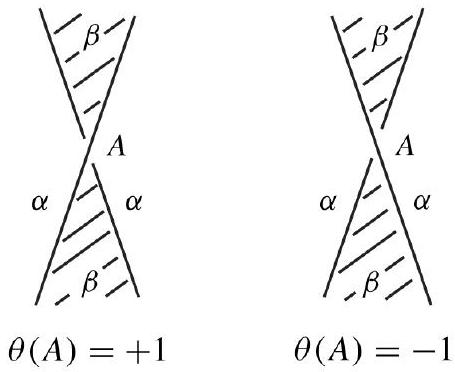
\includegraphics[scale=0.2, center]{2025_05_21_9c06be8de7a55410f8c1g-032}

Figure 2.5. The index $\theta(A)= \pm 1$.\\
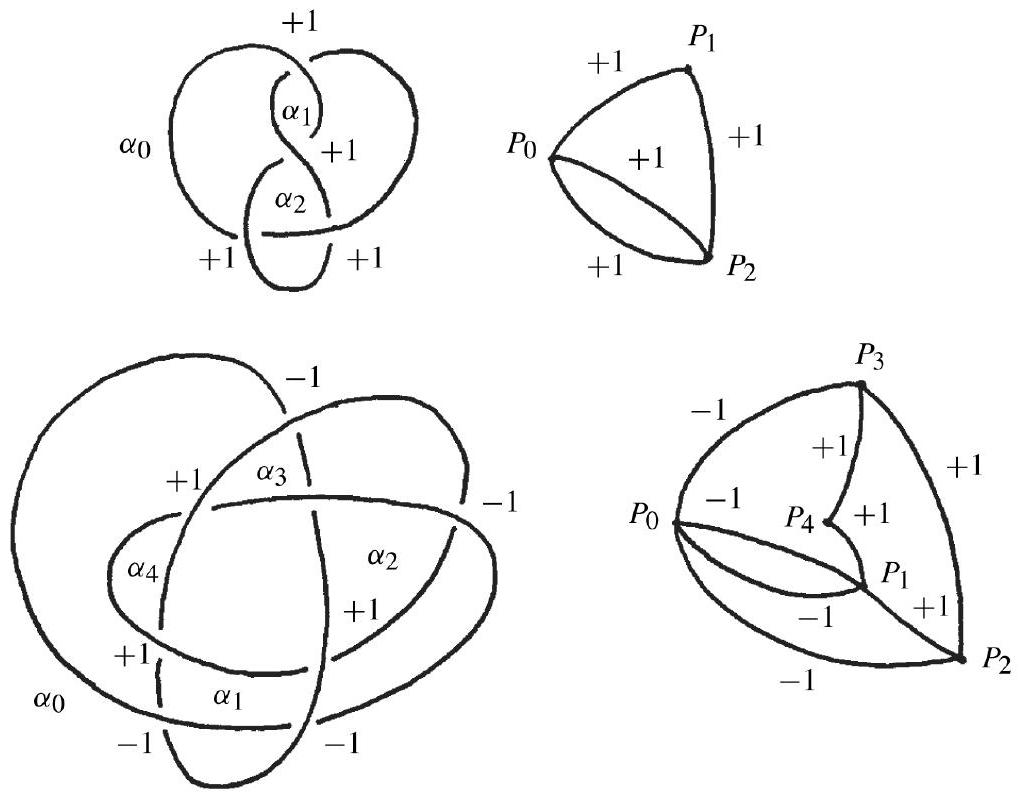
\includegraphics[scale=0.2, center]{2025_05_21_9c06be8de7a55410f8c1g-033}

Figure 2.6\\
a projection is alternating if and only if the index function $\theta(A)$ on the double points is a constant (Figure 2.6).

Graphs of knots have been repeatedly employed in knot theory [12], [76], [196]. We shall take up the subject again in Chapter 13 in connection with the quadratic form of a knot.
\end{DEF}

\begin{DEF}{KNO-B14-02-33}{Komplement des Knoten}
$V=V(\mathfrak{k})$ denotes a tubular neighborhood of the knot $\mathfrak{k}$ and $C=\overline{S^{3}-V}$ is called the complement of the knot. $H_{j}$ will denote the (singular) homology with coefficients in $\mathbb{Z}$.
\end{DEF}

\subsection{Knotengruppe und Wirtinger Präsentation}

\begin{CONC}{KNO-B14-03-06}{Wirtinger Prozedur}
Embed the knot $\mathfrak{k}$ into $\mathbb{R}^{3}$ such that its projection onto the plane $\mathbb{R}^{2}$ is regular. The projecting cylinder $Z$ has self-intersections in $n$ projecting rays $a_{i}$ corresponding to the $n$ double points of the regular projection. The $a_{i}$ decompose $Z$ into $n$ 2-cells $Z_{i}$ (see Figure 3.1) where $Z_{i}$ is bounded by $a_{i-1}, a_{i}$ and the overcrossing arc $\sigma_{i}$ of $\mathfrak{k}$.

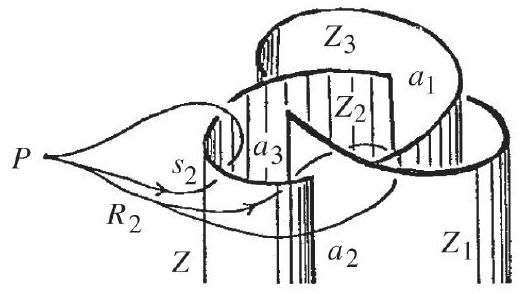
\includegraphics[scale=0.2,center]{2025_05_21_9c06be8de7a55410f8c1g-046}
Figure 3.1

Choose the orientation of $Z_{i}$ to induce on $\sigma_{i}$ the direction of $\mathfrak{k}$. The complement of $Z$ can be retracted parallel to the rays onto a half-space above the knot; thus it is contractible.

To compute $\pi_{1} C$ for some basepoint $P \in C$ observe that there is (up to a homotopy fixing $P$ ) exactly one polygonal closed path in general position relative to $Z$ which intersects a given $Z_{i}$ with intersection number $\varepsilon_{i}$ and which does not intersect the other $Z_{j}$. Paths of this type, taken for $i=1,2, \ldots, n$ and $\varepsilon_{i}=1$, represent generators $s_{i} \in \pi_{1} C$. To see this, let a path in general position with respect to $Z$ represent an arbitrary element of $\pi_{1} C$. Move its intersection points with $Z_{i}$ into the intersection of the curves $s_{i}$. Now the assertion follows since the complement of $Z$ is contractible. Running through an arbitrary closed polygonal path $\omega$ yields the homotopy class as a word $w\left(s_{i}\right)=s_{i_{1}}^{\varepsilon_{1}} \ldots s_{i_{r}}^{\varepsilon_{r}}$ if in turn each intersection with $Z_{i_{j}}$ and intersection number $\varepsilon_{j}$ is put down by writing $s_{i_{j}}^{\varepsilon_{j}}$.

To obtain relations, consider a small path $\varrho_{j}$ in $C$ encircling $a_{j}$ and join it with $P$ by an arc $\lambda_{j}$. Then $\lambda_{j} \varrho_{j} \lambda_{j}^{-1}$ is contractible and the corresponding word $l_{j} r_{j} l_{j}^{-1}$ in the generators $s_{i}$ is a relation. The word $r_{j}\left(s_{j}\right)$ can easily be read off from the knot projection. According to the characteristic $\eta \in\{1,-1\}$ of a double point, see Figure 3.2, we get the relation

$$
r_{j}=s_{j} s_{i}^{-\eta_{j}} s_{k}^{-1} s_{i}^{\eta_{j}} .
$$

\begin{center}
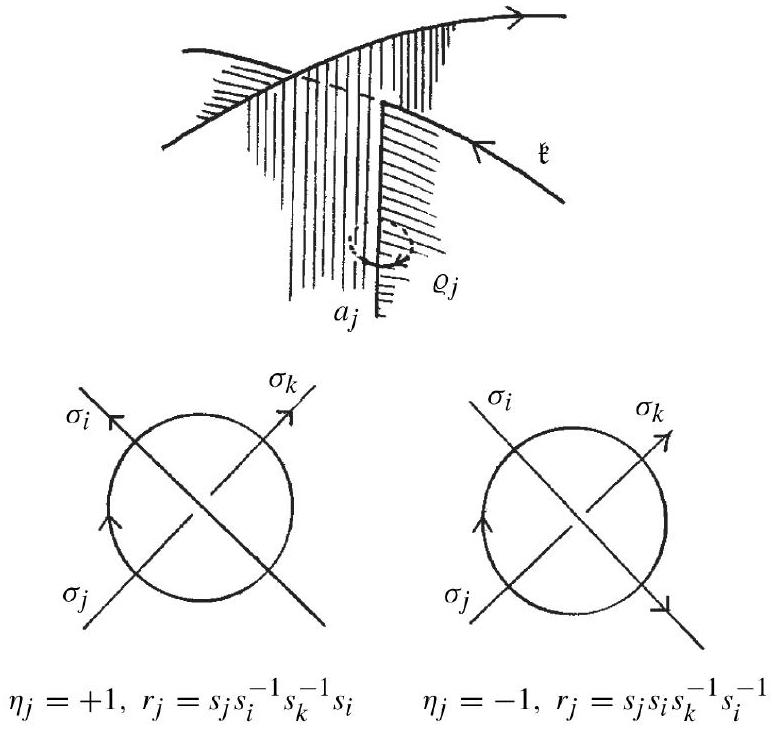
\includegraphics[scale=0.2]{2025_05_21_9c06be8de7a55410f8c1g-047}
\end{center}
Figure 3.2. The Wirtinger relations.
\end{CONC}

\begin{THEO}{KNO-B14-03-01}{Wirtinger Presentation}
Let $\sigma_{i}, i=1,2, \ldots, n$, be the overcrossing arcs of a regular projection of a knot (or link) $\mathfrak{k}$. Then the knot group admits the following so-called Wirtinger presentation:
$$
\mathfrak{G}=\pi_{1}\left(\overline{S^{3}-V(\mathfrak{f})}\right)=\left\langle s_{1}, \ldots, s_{n} \mid r_{1}, \ldots, r_{n}\right\rangle .
$$
The arc $\sigma_{i}$ corresponds to the generator $s_{i}$; a crossing of characteristic $\eta_{j}$ as in Figure 3.2 gives rise to the defining relations
$$
r_{j}=s_{j} s_{i}^{-\eta_{j}} s_{k}^{-1} s_{i}^{\eta_{j}} .
$$
\end{THEO}

\begin{PROOF}{KNO-B14-03-02}{P: Wirtinger Presentation}
It remains to check that $r_{1}, \ldots, r_{n}$ are defining relations. Consider $\mathbb{R}^{3}$ as a simplicial complex $\Sigma$ containing $Z$ as a subcomplex, and denote by $\Sigma^{*}$ the dual complex. Let $\omega$ be a contractible curve in $C$, starting at a vertex $P$ of $\Sigma^{*}$. By simplicial approximation $\omega$ can be replaced by a path in the 1 -skeleton of $\Sigma^{*}$ and the contractible homotopy by a series of homotopy moves which replace arcs on the boundary of 2-cells $\sigma^{2}$ of $\Sigma^{*}$ by the inverse of the rest. If $\sigma^{2} \cap Z=\emptyset$ the deformation over $\sigma^{2}$ has no effect on the words $\omega\left(s_{i}\right)$. If $\sigma^{2}$ meets $Z$ in an arc then the deformation over $\sigma^{2}$ either cancels or inserts a word $s_{i}^{\varepsilon} s_{i}^{-\varepsilon}, \varepsilon \in\{1,-1\}$, in $\omega\left(s_{i}\right)$; hence, it does not affect the element of $\pi_{1} C$ represented by $\omega$. If $\sigma^{2}$ intersects a double line $a_{j}$ then the deformation over $\sigma^{2}$ omits or inserts a relation: a conjugate of $r_{j}$ or $r_{j}^{-1}$ for some $j$.
\end{PROOF}

\begin{PROP}{KNO-B14-03-04}{Fundamentalgruppe des Komplements von tabularen Umgebungen charakterisiert den trivialen Knoten}
If $\mathfrak{k}$ is a non-trivial knot the inclusion $i: \partial V \rightarrow C=\overline{S^{3}-V}$ induces an injective homomorphism $i_{\#}: \pi_{1} \partial V \rightarrow \pi_{1} C$. In particular, if $\pi_{1} C \cong \mathbb{Z}$ is cyclic then the knot $\mathfrak{k}$ is trivial.
\end{PROP}

\begin{PROOF}{KNO-B14-03-05}{P: Fundamentalgruppe des Komplements von tabularen Umgebungen charakterisiert den trivialen Knoten}
Suppose $i_{\#}$ is not injective. Then the Loop Theorem of Papakyriakopoulos [281], see Appendix B.5 [159, 4.2], guarantees the existence of a simple closed curve $\kappa$ on $\partial V$ and a disk $\delta$ in $C$ such that
$$
\kappa = \partial \delta 
\quad \text{(hence } \kappa \simeq 0 \text{ in } C\text{),} \quad 
\delta \cap V = \kappa \quad \text{and} \quad 
\kappa \not\simeq 0 \text{ in } \partial V\text{.}
$$
Since $\kappa$ is simple and $\kappa \sim 0$ in $C$ it is a longitude, see 3.2. So there is an annulus $A \subset V$ such that $A \cap \partial V=\kappa, \partial A=\kappa \cup \mathfrak{k}$, as has been shown in Theorem 3.1. This proves that $\mathfrak{k}$ bounds a disk in $S^{3}$ and, hence, is the trivial knot.
\end{PROOF}

\begin{KORO}{KNO-B14-03-03}{Relationen der Wirtinger Präsentation sind Konsequenz der anderen Relationen}
Let $\mathfrak{k}$ be a knot or link and $\left\langle s_{1}, \ldots, s_{n} \mid r_{1}, \ldots, r_{n}\right\rangle$ a Wirtinger presentation of $\mathfrak{G}$. Then each defining relation $r_{j}$ is a consequence of the other defining relations $r_{i}, i \neq j$.
\end{KORO}

\begin{PROOF}{KNO-B14-03-07}{P: Relationen der Wirtinger Präsentation sind Konsequenz der anderen Relationen}
Choose the curves $\lambda_{j} \varrho_{j} \lambda_{j}^{-1}$ (see the paragraph before Theorem 3.4) in a plane $E$ parallel to the projection plane and "far down" such that $E$ intersects all $a_{i}$. Let $\delta$ be a disk in $E$ such that $\mathfrak{k}$ is projected into $\delta$, and let $\gamma$ be the boundary of $\delta$. We assume that $P$ is on $\gamma$ and that the $\lambda_{j}$ have only the basepoint $P$ in common. Then, see Figure 3.3,
$$
\gamma \simeq \prod_{j=1}^{n} \lambda_{j} \varrho_{j} \lambda_{j}^{-1} \quad \text { in } E-\left(\bigcup_{j} a_{j} \cap E\right)
$$
\begin{center}
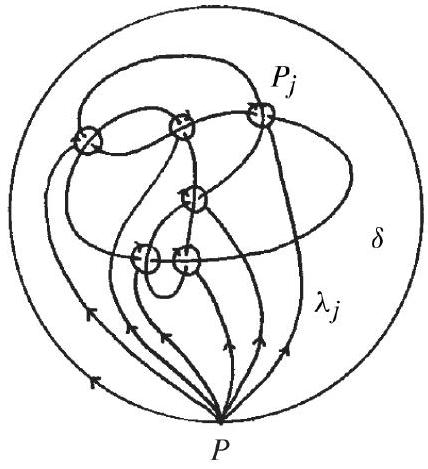
\includegraphics[scale=0.2]{2025_05_21_9c06be8de7a55410f8c1g-049}
\end{center}
Figure 3.3

This implies the equation
$$
1 \equiv \prod_{j=1}^{n} l_{j} r_{j} l_{j}^{-1}
$$
in the free group generated by the $s_{i}$, where $l_{j}$ is the word which corresponds to $\lambda_{j}$. Thus each relation $r_{j}$ is a consequence of the other relations.
\end{PROOF}

\subsection{Hurewicz-Abbildung}

\begin{CONC}{AT-H09-02-04}{Herleitung der Hurewicz-Abbildung}
Es sei $n \geq 1$. Nach Satz IV.9.5 ist $H_n\left(S^n\right) \cong \mathbb{Z}$, die Gruppe $H_n\left(S^n\right)$ besitzt daher zwei Erzeuger. Wir fixieren einen dieser Erzeuger $\alpha_n \in H_n\left(S^n\right)$, nämlich den aus Proposition IV.9.9, und bezeichnen ihn von nunan als den Standarderzeuger von $H^n\left(S^n\right)$.

Ist $\sigma: S^n \rightarrow X$ eine stetige Abbildung so erhalten wir eine Homologieklasse $\sigma_*\left(\alpha_n\right) \in H_n(X)$. Nach Korollar IV.7.5 hängt diese Homotopieklasse nur von der Homotopieklasse von $\sigma$ ab, die Konstruktion liefert daher eine wohldefinierte Abbildung
$$
\tilde{h}_n=\tilde{h}_n^X:\left[S^n, X\right] \rightarrow H_n(X), \quad \tilde{h}_n([\sigma]):=\sigma_*\left(\alpha_n\right) .
$$
Diese Abbildung ist natürlich, dh. für jede stetige Abbildung $f: X \rightarrow Y$ kommutiert das Diagramm
\[
\begin{tikzcd}
{[S^n, X]} \arrow[r, "\tilde{h}_n^X"] \arrow[d, "f_*"'] & H_n(X) \arrow[d, "f_*"] \\
{[S^n, Y]} \arrow[r, "\tilde{h}_n^Y"'] & H_n(Y)
\end{tikzcd}
\]
wobei die Abbildung $f_*:\left[S^n, X\right] \rightarrow\left[S^n, Y\right]$ durch $f_*([\sigma])=$ $[f \circ \sigma]$ gegeben ist, vgl. Bemerkung I.3.6. 

Um dies einzusehen betrachten wir eine beliebige stetige Abbildung $\sigma: S^n \rightarrow X$. Aus der Funktorialität der Homologie erhalten wir sofort 
$$\tilde{h}_n^Y\left(f_*([\sigma])\right)=\tilde{h}_n^Y([f \circ \sigma])=(f \circ \sigma)_*\left(\alpha_n\right)=f_*\left(\sigma_*\left(\alpha_n\right)\right)=f_*\left(\tilde{h}_n^X([\sigma])\right)$$ 
Wir werden uns im Folgenden auf den Fall $n=1$ beschränken.

Es sei nun $(X, x_0)$ ein punktierter Raum. Wir werden im Folgenden die Beschreibung der Fundaentalgruppe aus Proposition I.3.32 verwenden, $\pi_1\left(X, x_0\right)=$ $\left[\left(S^1, 1\right),\left(X, x_0\right)\right]$. Wir haben in Satz I.3.33 die Abbildung $\Phi_{\left(X, x_0\right)}: \pi_1\left(X, x_0\right) \rightarrow$ [ $S^1, X$ ] studiert, die einer Homotopieklasse von Schleifen bei $x_0$ die zugrundeliegende freie Homotopieklasse zuordnet. Setzen wir diese mit $\tilde{h}_1^X$ zusammen, erhalten wir eine Abbildung
$$
h_1=h_1^{\left(X, x_0\right)}: \pi_1\left(X, x_0\right) \rightarrow H_1(X), \quad h_1([\sigma]):=\sigma_*\left(\alpha_1\right) .
$$
Diese Abbildung wird der (erste) Hurewicz-Homomorphismus genannt.
\end{CONC}

\begin{LEM}{AT-H09-02-05}{Diagonalabbildung und Inklusionsstruktur in $H_1\left(S^1 \vee S^1\right)$}
Die Abbildung $\mu: S^1 \longrightarrow S^1 \vee S^1$ induzierten den Homomorphismus $\mu_*: H_1(S^1) \longrightarrow H_1(S^1 \vee S^1)$. Für $\alpha \in H_1\left(S^1\right)$ gilt $\mu_*(\alpha)=\left(\iota_1\right)_*(\alpha)+\left(\iota_2\right)_*(\alpha)$, wobei $\iota_1, \iota_2: S^1 \rightarrow S^1 \vee S^1$ die beiden kanonischen Inklusionen bezeichnen. In anderen Worten, das folgende Diagramm kommutiert:
\[
\begin{tikzcd}
H_1(S^1) \arrow[r, "\mu_*"] \arrow[dr, "\Delta"'] & H_1(S^1 \vee S^1) \\
& H_1(S^1) \oplus H_1(S^1) \arrow[u, "(\iota_1)_* + (\iota_2)_*"', "\cong"]
\end{tikzcd}
\]
Dabei bezeichnet 
$$\left(\iota_1\right)_*+\left(\iota_2\right)_*: H_1\left(S^1\right) \oplus H_1\left(S^1\right) \stackrel{\cong}{\rightarrow} H_1\left(S^1 \vee S^1\right)$$ 
den von den beiden Inklusionen $\iota_1, \iota_2: S^1 \rightarrow S^1 \vee S^1$ induzierten Isomorphimus, siehe Beispiel IV.9.11, und $\Delta: H_1\left(S^1\right) \rightarrow H_1\left(S^1\right) \oplus H_1\left(S^1\right)$ bezeichnet die Diagonalabbildung, $\Delta(\alpha):=(\alpha, \alpha)$, ein Homomorphismus.
\end{LEM}

\begin{PROOF}{AT-H09-02-06}{P: Diagonalabbildung und Inklusionsstruktur in $H_1\left(S^1 \vee S^1\right)$}
Wir betrachten die beiden Abbildungen $p_1, p_2: S^1 \vee S^1 \rightarrow S^1$, die durch $p_1 \circ \iota_1=\operatorname{id}_{S^1}=p_2 \circ \iota_2$ und $p_2 \circ \iota_1=c=p_1 \circ \iota_2$ vollständig bestimmt sind. Dabei bezeichnet $c: S^1 \rightarrow S^1, c(z):=1$, die konstante Abbildung. Es gilt daher $\left(p_1\right)_* \circ\left(\iota_1\right)_*=\operatorname{id}_{H_1\left(S^1\right)}=\left(p_2\right)_* \circ\left(\iota_2\right)_*$ sowie $\left(p_2\right)_* \circ\left(\iota_1\right)_*=0=\left(p_1\right)_* \circ\left(\iota_2\right)_*$. Aus diesen Relationen sehen wir, dass
$$
\left(\left(p_1\right)_*,\left(p_2\right)_*\right): H_1\left(S^1 \vee S^1\right) \stackrel{\cong}{\rightrightarrows} H_1\left(S^1\right) \oplus H_1\left(S^1\right)
$$
invers zu dem von den Inklusionen induzierten Isomorphismus $\left(\iota_1\right)_*+\left(\iota_2\right)_*$ ist. Es genügt daher $\left(\left(p_1\right)_*,\left(p_2\right)_*\right) \circ \mu_*=\Delta$ zu zeigen. Dies ist offensichtlich zu den beiden Gleichungen $\left(p_1\right)_* \circ \mu_*=\operatorname{id}_{H_1\left(S^1\right)}=\left(p_2\right)_* \circ \mu_*$ äquivalent. Aus der expliziten Gestalt von $\mu$, siehe (I.5), folgt $p_1 \circ \mu \simeq \operatorname{id}_{S^1} \simeq p_2 \circ \mu$, und dies impliziert die gewünschten Relationen.
\end{PROOF}

\begin{PROP}{AT-H09-02-07}{Hurewicz-Abbildung ist ein natürlicher Homomorphismus}
Ist $(X, x_0)$ ein punktierter Raum, dann definiert 
$$h_1=h_1^{\left(X, x_0\right)}: \pi_1\left(X, x_0\right) \rightarrow H_1(X), \quad h_1([\sigma]):=\sigma_*\left(\alpha_1\right)$$
einen Gruppenhomomorphismus. Dieser Homomorphismus ist natürlich, dh. das Diagramm
% Linkes Diagramm
\[
\begin{tikzcd}
\pi_1(X, x_0) \arrow[r, "h_1^{(X,x_0)}"] \arrow[d, "f_*"'] & H_1(X) \arrow[d, "f_*"] \\
\pi_1(Y, y_0) \arrow[r, "h_1^{(Y,y_0)}"'] & H_1(Y)
\end{tikzcd}
\]
kommutiert für jede Abbildung punktierter Räume $f:\left(X, x_0\right) \rightarrow\left(Y, y_0\right)$. 

Für jeden Weg $h: I \rightarrow X$ von $h(0)=x_0$ nach $h(1)=x_1$ ist darüber hinaus das rechte Diagramm oben kommutative, siehe Proposition I.1.18
\[
\begin{tikzcd}
  & H_1(X) \arrow[dl, "h_1^{(X,x_0)}"'] \arrow[dr, "h_1^{(X,x_1)}"] \\
  \pi_1(X, x_0) \arrow[rr, "\beta_h"', "\cong"{above}] & & \pi_1(X, x_1)
\end{tikzcd}
\]
\end{PROP}

\begin{PROOF}{AT-H09-02-08}{P: Hurewicz-Abbildung ist ein natürlicher Homomorphismus}
Sind $\sigma_1, \sigma_2: I \rightarrow X$ zwei Schleifen bei $x_0$, dann folgt aus Lemma IV.11.1(iv)
$$
h_1\left(\left[\sigma_1\right]\left[\sigma_2\right]\right)=h_1\left(\left[\sigma_1 \sigma_2\right]=\left[\left(\sigma_1 \sigma_2\right)^{\sim}\right]=\left[\tilde{\sigma}_1\right]+\left[\tilde{\sigma}_2\right]=h_1\left(\left[\sigma_1\right]\right)+h_1\left(\left[\sigma_2\right]\right),\right.
$$
also ist (IV.43) ein Gruppenhomomorphismus. Ist $f:\left(X, x_0\right) \rightarrow\left(Y, y_0\right)$ eine Abbildung punktierter Räume und $\sigma: I \rightarrow X$ eine Schleife bei $x_0$, dann folgt aus Lemma IV.11.1(vi)
$$
\begin{aligned}
h_1^{\left(Y, y_0\right)}\left(f_*([\sigma])\right)=h_1^{\left(Y, y_0\right)}([f \circ \sigma])=\left[(f \circ \sigma)^{\sim}\right] & \\
& =[f \circ \tilde{\sigma}]=f_*([\tilde{\sigma}])=f_*\left(h_1^{\left(X, x_0\right)}([\sigma])\right)
\end{aligned}
$$
Dies zeigt die Natürlichkeit von $h_1$. Ist nun $\sigma: I \rightarrow X$ eine Schleife bei $x_1$, dann folgt
$$
\begin{aligned}
h_1^{\left(X, x_0\right)}\left(\beta_h([\sigma])\right)=h_1^{\left(X, x_0\right)}([h \sigma \bar{h}]) & =\left[(h \sigma \bar{h})^{\sim}\right] \\
= & {\left[\tilde{h}+\tilde{\sigma}+\bar{h}^{\sim}\right]=[\tilde{h}+\tilde{\sigma}-\tilde{h}]=[\tilde{\sigma}]=h_1^{\left(X, x_0\right)}([\sigma]) }
\end{aligned}
$$
wobei wir Lemma IV.11.1(iv) und (v) verwendet haben.
\end{PROOF}

\begin{PROP}{AT-H09-02-09}{Hurewicz-Homomorphismus induziert einen Isomorphismus für abelisierte Fundamentalgruppe für WZSH punktierte Räume}
Es sei $(X, x_0)$ ein wegzusammenhängender punktierter Raum. Dann ist der Hurewicz-Homomorphismus 
$$\tilde{h}_n=\tilde{h}_n^X:\left[S^n, X\right] \rightarrow H_n(X), \quad \tilde{h}_n([\sigma]):=\sigma_*\left(\alpha_n\right)$$
surjektiv und sein Kern stimmt mit der Kommutatoruntergruppe von $\pi_1\left(X, x_0\right)$ überein. Er induziert daher einen Isomorphismus $\pi_1\left(X, x_0\right)_{\mathrm{ab}} \cong H_1(X)$.
\end{PROP}

\begin{PROOF}{AT-H09-02-10}{P: Hurewicz-Homomorphismus induziert einen Isomorphismus für abelisierte Fundamentalgruppe für WZSH punktierte Räume}
Da $H_1(X)$ abelsch ist, induziert (IV.43) einen Homomorphismus
$$
h_1: \pi_1\left(X, x_0\right)_{\mathrm{ab}} \rightarrow H_1(X)
$$
es genügt zu zeigen, dass (IV.44) ein Isomorphismus ist. Da $X$ wegzusammenhängend ist, können wir zu jedem Punkt $x \in X$ einen Weg $\rho_x: I \rightarrow X$ von $\rho_x(0)=x_0$ nach $\rho_x(1)=x$ wählen. Ist nun $\tilde{\sigma}: \Delta^1 \rightarrow X$ ein 1-Simplex und $\sigma: I \rightarrow X$ der entsprechende Weg, dann ist $\left(\rho_{\sigma(0)} \sigma\right) \bar{\rho}_{\sigma(1)}$ eine Schleife bei $x_0$ und definiert daher ein Element in $\left[\rho_{\sigma(0)} \sigma \bar{\rho}_{\sigma(1)}\right] \in \pi_1\left(X, x_0\right)$. Da $\pi_1\left(X, x_0\right)_{\text {ab }}$ abelsch ist können wir einen Homomorphismus auf Erzeugern $\tilde{\sigma}: \Delta^1 \rightarrow X$ wie folgt definieren:
$$
\phi: C_1(X) \rightarrow \pi_1\left(X, x_0\right)_{\mathrm{ab}}, \quad \phi(\tilde{\sigma}):=\left[\rho_{\sigma(0)} \sigma \bar{\rho}_{\sigma(1)}\right] .
$$
Wir zeigen zunächst
$$
\phi \circ \partial=1: C_2(X) \rightarrow \pi_1\left(X, x_0\right)_{\mathrm{ab}}
$$
dh. $\phi$ definiert einen Homomorphismus
$$
\phi: H_1(X) \rightarrow \pi_1\left(X, x_0\right)_{\mathrm{ab}}, \quad \phi([c]):=\phi(c) .
$$
Für $\tau: \Delta^2 \rightarrow X$ ist also $\phi(\partial \tau)=1$ zu zeigen. ${ }^{37}$ Setzen wir $\tilde{\sigma}_i:=\tau \circ \delta_2^i: \Delta^1 \rightarrow X$, $i=0,1,2$, dann gilt offensichtlich $\partial \tau=\tilde{\sigma}_0-\tilde{\sigma}_1+\tilde{\sigma}_2$. Da $\phi$ ein Homomorphismus ist, erhalten wir:
$$
\begin{aligned}
\phi(\partial \tau) & =\phi\left(\tilde{\sigma}_0\right) \phi\left(\tilde{\sigma}_1\right)^{-1} \phi\left(\tilde{\sigma}_2\right) \\
& =\left[\rho_{\sigma_0(0)} \sigma_0 \bar{\rho}_{\sigma_0(1)}\right]\left[\rho_{\sigma_1(0)} \sigma_1 \bar{\rho}_{\sigma_1(1)}\right]^{-1}\left[\rho_{\sigma_2(0)} \sigma_2 \bar{\rho}_{\sigma_2(1)}\right] \\
& =\left[\rho_{\sigma_0(0)} \sigma_0 \bar{\rho}_{\sigma_0(1)} \rho_{\sigma_1(1)} \bar{\sigma}_1 \bar{\rho}_{\sigma_1(0)} \rho_{\sigma_2(0)} \sigma_2 \bar{\rho}_{\sigma_2(1)}\right] \\
& =\left[\rho_{\sigma_0(0)} \sigma_0 \bar{\sigma}_1 \sigma_2 \bar{\rho}_{\sigma_2(1)}\right] \\
& =\left[\rho_{\sigma_0(0)} \bar{\rho}_{\sigma_2(1)}\right]=\left[c_{x_0}\right]=1
\end{aligned}
$$
Dabei haben wir verwendet, dass $\sigma_0 \bar{\sigma}_1 \sigma_2, \bar{\rho}_{\sigma_0(1)} \rho_{\sigma_1(1)}, \bar{\rho}_{\sigma_1(0)} \rho_{\sigma_2(0)}$ und $\rho_{\sigma_0(0)} \bar{\rho}_{\sigma_2(1)}$ nullhomotope Schleifen sind. Damit ist (IV.45) gezeigt. Es genügt nun zu zeigen, dass (IV.46) invers zu (IV.44) ist. Zunächst gilt
$$
\phi \circ h_1=\operatorname{id}_{\pi_1\left(X, x_0\right)_{\mathrm{ab}}}
$$
denn für jede Schleife $\sigma: I \rightarrow X$ bei $x_0$ gilt
$$
\phi\left(h_1([\sigma])\right)=\phi([\tilde{\sigma}])=\phi(\tilde{\sigma})=\left[\rho_{x_0} \sigma \bar{\rho}_{x_0}\right]=\left[\rho_{x_0}\right][\tilde{\sigma}]\left[\rho_{x_0}\right]^{-1}=[\sigma]
$$

Es bleibt daher nur noch
$$
h_1 \circ \phi=\operatorname{id}_{H_1(X)}
$$
zu zeigen. Um dies einzusehen definieren wir einen Homomorphismus auf Erzeugern $x \in X$ durch
$$
g: C_0(X) \rightarrow C_1(X), \quad g(x):=\tilde{\rho}_x
$$
Für jeden 1-Simplex $\tilde{\sigma}: \Delta^1 \rightarrow X$ gilt dann
$$
\begin{aligned}
h_1(\phi(\tilde{\sigma}))= & h_1\left(\left[\rho_{\sigma(0)} \sigma \bar{\rho}_{\sigma(1)}\right]\right)=\left[\left(\rho_{\sigma(0)} \sigma \bar{\rho}_{\sigma(1)}\right)^{\sim}\right] \\
& =\left[\tilde{\rho}_{\sigma(0)}+\tilde{\sigma}-\tilde{\rho}_{\sigma(1)}\right]=[\tilde{\sigma}-g(\partial \tilde{\sigma})] .
\end{aligned}
$$
Dabei haben wir Lemma IV.11.1(iv) und (v) verwendet. Es folgt sofort $h_1(\phi(c))=$ $[c-g(\partial c)]$ für alle $c \in C_1(X)$, also $h_1(\phi(c))=[c]$, für alle Zyklen $c \in Z_1(X)$. Damit ist (IV.47) gezeigt und der Beweis vollständig.
\end{PROOF}

\begin{LEM}{AT-H09-02-02}{Homologische Eigenschaften von Wegen}
Es gilt:
\begin{enumerate}[label=(\roman*)]
    \item Punkte erzeugen in Homologie keine nichttrivialen 1-Zykel: Ist $x \in X$, dann existiert $\tau \in C_2(X)$ mit $\tilde{c}_x = \partial \tau$.${}^{35}$
    
    \item Der Rand einer Schleife ist Null: Ist $\sigma: I \rightarrow X$ eine Schleife, dann gilt $\partial \tilde{\sigma} = 0$.
    
    \item Homotope Wege sind homolog: Sind $\sigma_0 \simeq \sigma_1: I \rightarrow X$ homotop relativ Endpunkten, dann existiert $\tau \in C_2(X)$ mit $\tilde{\sigma}_1 = \tilde{\sigma}_0 + \partial \tau$.
    
    \item Konkatenation ergibt Summe plus Rand: Sind $\sigma_0, \sigma_1: I \rightarrow X$ mit $\sigma_0(1) = \sigma_1(0)$, dann existiert $\tau \in C_2(X)$ mit $\left( \sigma_0 \sigma_1 \right)^{\sim} = \tilde{\sigma}_0 + \tilde{\sigma}_1 + \partial \tau$.
    
    \item Inversion ist bis auf Vorzeichen und Rand eindeutig: Ist $\sigma: I \rightarrow X$, dann existiert $\tau \in C_2(X)$ mit $\bar{\sigma}^{\sim} = -\tilde{\sigma} + \partial \tau$.${}^{36}$
    
    \item Stetige Abbildungen vertragen sich mit Tildefizierung: Ist $f: X \rightarrow Y$ stetig und $\sigma: I \rightarrow X$, dann gilt $f \circ \tilde{\sigma} = (f \circ \sigma)^{\sim}$.
\end{enumerate}
\end{LEM}

\begin{PROOF}{AT-H09-02-03}{P: Homologische Eigenschaften von Wegen}
Ad (i): Für den konstanten 2-Simplex $\tau: \Delta^2 \rightarrow X, \tau\left(t_0, t_1, t_2\right):=x$, erhalten wir $\partial \tau=\tilde{c}_x-\tilde{c}_x+\tilde{c}_x=\tilde{c}_x$. 

Ad (ii): Für eine Schleife $\sigma: I \rightarrow X$ gilt $\partial \tilde{\sigma}=$ $\sigma(1)-\sigma(0)=0 \in C_0(X)$. 

Ad (iii): Sei also $H: I \times I \rightarrow X$ eine Homotopie relativ Endpunkten von $\sigma_0$ nach $\sigma_1$. Definiere $x_0:=\sigma_0(0)=\sigma_1(0), x_1:=\sigma_0(1)=\sigma_1(1)$, $\rho: I \rightarrow X, \rho(t):=H_t(t)$, sowie $\tau_0, \tau_1: \Delta^2 \rightarrow X, \tau_0\left(t_0, t_1, t_2\right):=H_{t_2}\left(t_1+t_2\right)$, $\tau_1\left(t_0, t_1, t_2\right):=H_{t_1+t_2}\left(t_2\right)$. Dann gilt $\partial \tau_0=\tilde{c}_{x_1}-\tilde{\rho}+\tilde{\sigma}_0$ und $\partial \tau_1=\tilde{\sigma}_1-\tilde{\rho}+\tilde{c}_{x_0}$. Nach (i) existieren $\tau_2, \tau_3 \in C_2(X)$ mit $\partial \tau_2=\tilde{c}_{x_0}$ und $\partial \tau_3=\tilde{c}_{x_1}$. Wir erhalten daher
$$
\tilde{\sigma}_1-\tilde{\sigma}_0=\partial\left(\tau_1-\tau_0-\tau_2+\tau_3\right)
$$
die Behauptung folgt daher mit $\tau:=\tau_1-\tau_0-\tau_2+\tau_3$. 

Ad (iv): Definieren wir $\tau: \Delta^2 \rightarrow X, \tau\left(t_0, t_1, t_2\right):=\left(\sigma_0 \sigma_1\right)\left(t_1 / 2+t_2\right)$, dann folgt $\partial \tau=\tilde{\sigma}_1-\left(\sigma_0 \sigma_1\right)^{\sim}+\tilde{\sigma}_0$. $\operatorname{Ad}(\mathrm{v})$ : Setze $x_0:=\sigma(0)$. Nach (iv) existiert $\tau_1 \in C_2(X)$ mit $(\sigma \bar{\sigma})^{\sim}=\tilde{\sigma}+\bar{\sigma}^{\sim}-\partial \tau$. Da $\sigma \bar{\sigma} \simeq c_{x_0}$ erhalten wir aus (iii) ein $\tau_2 \in C_2(X)$ mit $(\sigma \bar{\sigma})^{\sim}=\tilde{c}_{x_0}+\partial \tau_2$. Nach (i) existiert $\tau_3 \in C_2(X)$ mit $\partial \tau_3=\tilde{c}_{x_0}$. Zusammen erhalten wir
$$
\tilde{\sigma}+\bar{\sigma}^{\sim}=\partial\left(\tau_1+\tau_2+\tau_3\right) .
$$

Behauptung (vi) ist trivial, $(f \circ \tilde{\sigma})\left(t_0, t_1\right)=f\left(\tilde{\sigma}\left(t_0, t_1\right)\right)=f\left(\sigma\left(t_1\right)\right)=(f \circ \sigma)\left(t_1\right)=$ $(f \circ \sigma)^{\sim}\left(t_0, t_1\right)$, für $\left(t_0, t_1\right) \in \Delta^1$.
Nach Lemma IV.11.1(ii) und (iii) ist
$$
h_1=h_1^{\left(X, x_0\right)}: \pi_1\left(X, x_0\right) \rightarrow H_1(X), \quad h_1([\sigma]):=[\tilde{\sigma}] .
$$
eine wohldefinierte Abbildung, sie wird der (erste) Hurewicz-Homomorphismus genannt. Dabei bezeichnet $[\sigma] \in \pi_1\left(X, x_0\right)$ die Homotopieklasse der Schleife $\sigma$ : $I \rightarrow X$ bei $x_0$, und $[\tilde{\sigma}] \in H_1(X)$ die von dem ensprechenden 1-Simplex $\tilde{\sigma}$ : $\Delta^1 \rightarrow X$ repräsenterte Homologieklasse. In Proposition IV.11.2 unten werden wir zeigen, dass dies tatsächlich ein Gruppenhomomorphismus ist.
\end{PROOF}

\subsection{1. Homologiegruppe}

\begin{PROP}{KNO-B14-04-03}{Homologie des Knotenkomplements}
Let \( C = \overline{S^3 \setminus V} \) be the complement of the knot. We consider singular homology with integer coefficients, i.e., \( H_j = H_j(-; \mathbb{Z}) \). Then:
\[
H_j(C) \cong
\begin{cases}
\mathbb{Z} & \text{if } j = 0 \text{ or } j = 1, \\
0 & \text{otherwise}.
\end{cases}
\]
\end{PROP}

\begin{PROOF}{KNO-B14-04-04}{Homologie des Knotenkomplements}
Here we present one based on homological methods. We use the following well-known results:
$$
H_{n}\left(S^{3}\right)= \begin{cases}\mathbb{Z} & \text { for } n=0,3 \\ 0 & \text { otherwise }\end{cases}
$$
$$
\begin{aligned}
H_{n}(\partial V) & = \begin{cases}\mathbb{Z} & \text { for } n=0,2 \\
\mathbb{Z} \oplus \mathbb{Z} & \text { for } n=1, \\
0 & \text { otherwise, }\end{cases} \\
H_{n}(V)=H_{n}\left(S^{1}\right)= & \begin{cases}\mathbb{Z} & \text { for } n=0,1, \\
0 & \text { otherwise; }\end{cases}
\end{aligned}
$$
they can be found in standard books on algebraic topology, see Spanier [341], StöckerZieschang [346], Hatcher [157].

Since $C$ is connected, $H_{0}(C)=\mathbb{Z}$. For further calculations we use the MayerVietoris sequence of the pair ( $V, C$ ) where $V \cup C=S^{3}, V \cap C=\partial V$ :
\[
\begin{tikzcd}[row sep=small, column sep=small]
H_3(\partial V) \arrow[r] \arrow[d, equal] 
  & H_3(V) \arrow[r, phantom, "\oplus"] \arrow[d, equal] 
  & H_3(C) \arrow[r] 
  & H_3(S^3) \arrow[r] \arrow[d, "\cong", "\mathbb{Z}"']
  & H_2(\partial V) \arrow[r] \arrow[d, "\cong", "\mathbb{Z}"'] 
  & {} \\
0 & 0 & {} & \mathbb{Z} & \mathbb{Z} & {}
\end{tikzcd}
\]

\[
\begin{tikzcd}[row sep=small, column sep=small]
{} \arrow[r]
  & H_2(V) \arrow[r, phantom, "\oplus"] \arrow[d, equal]
  & H_2(C) \arrow[r] 
  & H_2(S^3) \arrow[r] \arrow[d, equal]
  & H_1(\partial V) \arrow[r] \arrow[d, "\cong"]
  & {} \\
{} & 0 & {}& 0 & \mathbb{Z} \oplus \mathbb{Z} & {}
\end{tikzcd}
\]

\[
\begin{tikzcd}[row sep=small, column sep=small]
{} \arrow[r] 
  & H_1(V) \arrow[r, phantom, "\oplus"] \arrow[d, "\cong"] & H_1(C) \arrow[r]
  & H_1(S^3) \arrow[d, equal] \\
{} & \mathbb{Z} & {} & 0
\end{tikzcd}
\]
It follows that $H_{1}(C)=\mathbb{Z}$. Since $\partial V$ is the boundary of the orientable compact 3manifold $C$, the group $H_{2}(\partial V)$ is mapped by the inclusion $\partial V \hookrightarrow C$ to $0 \in H_{2}(C)$. This implies that $H_{2}(C)=0$ and that $H_{3}\left(S^{3}\right) \rightarrow H_{2}(\partial V)$ is surjective; hence, $H_{3}(C)=0$.


Since $C$ is a 3-manifold it follows that $H_{n}(C)=0$ for $n>3$; this is also a consequence of the Mayer-Vietoris sequence.
\end{PROOF}

\subsection{Bemerkung zur Reichweite der Knotengruppe}

\begin{THEO}{KNO-F12-03-08}{Gordon–Luecke Theorem 1989}
If the complements of two tame knots are homeomorphic, then the knots are equivalent.
\end{THEO}

\begin{MOT}{KNO-F12-03-01}{Reichweite der Knotengruppe als Knoten Invariante}
Wir haben jetzt also eine Präsentation für $\pi_1\left(\mathbb{R}^3 \backslash K\right)$ gefunden. Aber was bringt uns das? Wir möchten gerne zeigen, dass $K$ nicht der triviale Knoten $T$ ist, d.h. das $\pi_1\left(\mathbb{R}^3 \backslash K\right) \neq \pi_1\left(\mathbb{R}^3 \backslash T\right)=\mathbb{Z}$. Die Präsentation von $\pi:=\pi_1\left(\mathbb{R}^3 \backslash K\right)$ schaut zwar kompliziert aus, aber vielleicht ist die Gruppe trotz allem isomorph zu $\mathbb{Z}$?
\end{MOT}

\begin{PROP}{KNO-F12-03-02}{Abelisierte Knotengruppe ist isomorph zu $\mathbb{Z}$}
Es sei $K \subset \mathbb{R}^3$ ein Knoten. Dann ist die Abelianisierung von $\pi_1\left(\mathbb{R}^3 \backslash K\right)$ isomorph zu $\mathbb{Z}$.
\end{PROP}

\begin{THEO}{KNO-F12-03-03}{Papakyriakopoulos 1975}
Ein Knoten $K \subset \mathbb{R}^3$ ist trivial, genau dann, wenn $\pi_1\left(\mathbb{R}^3 \backslash K\right) \cong \mathbb{Z}$.
\end{THEO}

\begin{CONC}{KNO-F12-03-04}{Word Problem für Präsentationen von Knotengruppen}
Es sei
$$
\pi=\left\langle g_1, \ldots, g_k \mid r_1, \ldots, r_l\right\rangle
$$
eine Präsentation einer Gruppe. Gibt es einen Algorithmus, welcher entscheiden kann, ob $\pi$ trivial ist oder isomorph zu $\mathbb{Z}$ ist?

Diese Frage ist als das 'word problem' bekannt, und wurde von Adyan und Rabin 1955 beantwort: Sie haben unabhängig von einander bewiesen, dass es solch einen Algorithmus nicht geben kann. Im Allgemeinen können wir also nicht entscheiden, ob eine gegebene Präsentation die Präsentation der trivialen Gruppe ist oder nicht.

Diese negative Aussage raubt uns erstmal alle Hoffnung, dass wir Fundamentalgruppen von Knotenkomplement verwenden können, um festzustellen, ob ein gegebener Knoten trivial ist oder nicht. Zum Glück ist unser Leben aber etwas einfacher: nicht jede Präsentation taucht als Präsentation der Fundamentalgruppe eines Knotenkomplements auf.
\end{CONC}

\begin{THEO}{KNO-F12-03-05}{Thurston 1982}
Es sei $K \subset \mathbb{R}^3$ ein nicht-trivialer Knoten, dann gibt es einen Epimorphismus $\pi_1\left(\mathbb{R}^3 \backslash K\right) \rightarrow G$ auf eine endliche nicht-kommutative Gruppe.
\end{THEO}

\begin{CONC}{KNO-F12-03-06}{Äquivalenz von Knoten bis auf Spiegelung}
Man kann sich nun auch fragen, ob zwei Knoten $K$ und $L$ genau dann äquivalent sind, wenn $\pi_1\left(\mathbb{R}^3 \backslash K\right) \cong \pi_1\left(\mathbb{R}^3 \backslash L\right)$. Dies ist im Allgemeinen jedoch nicht der Fall. Für einen Knoten $K$ bezeichnen wir mit $K^s$ das Spiegelbild von $K$ in der Ebene $(x, y, 0) \subset \mathbb{R}^3$, d.h.
$$
(x, y, z) \in K^s: \Leftrightarrow(x, y,-z) \in K .
$$
Dann sind $\mathbb{R}^3 \backslash K^s$ und $\mathbb{R}^3 \backslash K$ offensichtlich homöomorph, also besitzen sie die gleiche Fundamentalgruppe. Andererseits sind im Allgemeinen ein Knoten und sein Spiegelbild nicht äquivalent.

Wir können also jetzt etwas vorsichtiger fragen ob zwei Knoten $K$ und $L$ genau dann (bis auf Spiegelung) äquivalent sind, wenn $\pi_1\left(\mathbb{R}^3 \right.$ $K) \cong \pi_1\left(\mathbb{R}^3 \backslash L\right)$.

Um diese Frage zu diskutieren brauchen wir den Begriff der zusammenhängenden Summe $K \# L$ von orientierten Knoten $K$ und $L$, welcher in Abbildung 44 eingeführt wird. Wenn $K$ ein orientierter Knoten ist, dann bezeichnen wir mit $\bar{K}$ den gleichen Knoten mit umgekehrter Orientierung. Mithilfe des Satzes von Seifert-van Kampen kann man relativ leicht zeigen, dass für alle orientierten Knoten $K$ und $L$ gilt
$$
\pi_1\left(\mathbb{R}^3 \backslash K \# L\right) \cong \pi_1\left(\mathbb{R}^3 \backslash \bar{K} \# L\right),
$$
andererseits gibt es Knoten $K$ und $L$, so dass $\bar{K} \# L$ weder mit $K \# L$ noch mit dem Spiegelbild von $K \# L$ übereinstimmt.

Wir sagen nun, dass ein Knoten $K$ ein Primknoten ist, wenn $K$ nicht die zusammenhängende Summe von zwei nicht-trivialen Knoten ist. Folgender Satz wurde von Culler-Gordon-Luecke-Shalen-Witten ${ }^{96}$ bewiesen:
\end{CONC}

\begin{THEO}{KNO-F12-03-07}{Culler-Gordon-Luecke-Shalen-Witten 1989}
Es seien $K, J \subset \mathbb{R}^3$ zwei Primknoten mit $\pi_1\left(\mathbb{R}^3 \backslash K\right) \cong \pi_1\left(\mathbb{R}^3 \backslash J\right)$, dann gilt $K=J$ oder $K=J^s$.
\end{THEO}

\subsection{Äquivalente Charakterisierung der Fundamentalgruppe}

\begin{DEF}{AT-H09-04-01}{Homotopie zwischen stetigen Abbildungen}
Zwei stetige Abbildungen $f, g: X \rightarrow Y$ heißen homotop falls eine stetige Abbildung $H: X \times I \rightarrow Y$ mit $H_{0}=f$ und $H_{1}=g$ existiert. Dabei bezeichnet $H_{t}: X \rightarrow Y$ die stetige Abbildung $H_{t}(x):=H(x, t)$, $t \in I$. Jede solche Abbildung $H$ wird eine Homotopie von $f$ nach $g$ genannt. Wir schreiben $f \simeq g$ oder $f \stackrel{H}{\simeq} g$. Ist $f: X \rightarrow Y$ homotop zu einer konstanten Abbildung, dh. existiert $y_{0} \in Y$ mit $f \simeq c_{y_{0}}$ wobei $c_{y_{0}}: X \rightarrow Y, c_{y_{0}}(x):=y_{0}$, dann nennen wir $f$ nullhomotop.
\end{DEF}

\begin{DEF}{AT-H09-04-04}{Homotopieklassen von stetigen Abbildungen}
Die mit obiger Äquivalenzrelation assoziierten Äquivalenzklassen werden Homotopieklassen genannt. Die Menge der Homotopieklassen stetiger Abbildungen $X \rightarrow Y$ wird mit $[X, Y]$ bezeichnet. Die von $f: X \rightarrow Y$ repräsentierte Klasse werden wir mit $[f]$ bezeichnen.
\end{DEF}

\begin{DEF}{AT-H09-04-39}{Einpunktvereinigungen von punktierten Räumen}
Unter der Einpunktvereinigung zweier punktierter Räume $(X, x_{0})$ und $(Y, y_{0})$ verstehen wir den punktierten Raum der aus der disjunkten Vereinigung $X \sqcup Y$ durch Identifikation der beiden Punkte $x_{0}$ und $y_{0}$ ensteht. Genauer,
$$
\left(X, x_{0}\right) \vee\left(Y, y_{0}\right):=\left((X \sqcup Y) /\left\{x_{0}, y_{0}\right\}, *\right) .
$$
Die beiden Abbildungen punktierter Räume 
$$\iota_{X}:\left(X, x_{0}\right) \rightarrow\left(X, x_{0}\right) \vee\left(Y, y_{0}\right),\ \iota_{X}(x):=\left[\left(x, y_{0}\right)\right]$$ 
und 
$$\iota_{Y}:\left(Y, y_{0}\right) \rightarrow\left(X, x_{0}\right) \vee\left(Y, y_{0}\right),\ \iota_{Y}(y):=\left[\left(x_{0}, y\right)\right]$$ 
werden als kanonische Einbettungen bezeichnet. 

Beide sind Homöomorphismen auf ihr Bild, wir können daher ( $X, x_{0}$ ), und ebenso ( $Y, y_{0}$ ), als Teilraum von $\left(X, x_{0}\right) \vee\left(Y, y_{0}\right)$ auffassen.
\end{DEF}

\begin{CONC}{AT-H09-04-42}{Einpunktvereinigung von $S^1$ als Hilfsobjekte für alternative Beschreibung der Fundamentalgruppe}
Betrachte nun wieder $S^{1} \subseteq \mathbb{C}$ mit Basispunkt $1 \in S^{1}$. Weiters bezeichnen 
$$\iota_{1}:\left(S^{1}, 1\right) \rightarrow\left(S^{1}, 1\right) \vee\left(S^{1}, 1\right)$$ 
und 
$$\iota_{2}:\left(S^{1}, 1\right) \rightarrow\left(S^{1}, 1\right) \vee\left(S^{1}, 1\right)$$ 
die beiden kanonischen Inklusionen. Definiere Abbildungen punktierter Räume:
$$
\begin{array}{ll}
\mu:\left(S^{1}, 1\right) \rightarrow\left(S^{1}, 1\right) \vee\left(S^{1}, 1\right), & \mu(z):= \begin{cases}\iota_{1}\left(z^{2}\right) & \text { falls } \operatorname{Im} z \geq 0 \\
\iota_{2}\left(z^{2}\right) & \text { falls } \operatorname{Im} z \leq 0\end{cases} \\
\nu:\left(S^{1}, 1\right) \rightarrow\left(S^{1}, 1\right), & \nu(z):=z^{-1}=\bar{z}
\end{array}
$$
\end{CONC}

\begin{THEO}{AT-H09-04-43}{Natürliche Identifikation von $\left[\left(S^1, 1\right),\left(X, x_0\right)\right]$ mit $\pi_1\left(X, x_0\right)$}
Sei $(X, x_0)$ ein punktierter topologischer Raum. Dann gilt:
\begin{enumerate}
  \item \textbf{Definition der Abbildung:}
  \[
  \Psi = \Psi_{(X, x_0)} : \left[(S^1, 1), (X, x_0)\right] \longrightarrow \pi_1(X, x_0), \quad \Psi([f]) := [f \circ \omega_1],
  \]
  wobei $\omega_1 : I \to S^1$ die Standardparametrisierung des Einheitskreises ist.

  \item \textbf{Bijektivität:}  
  Die Abbildung $\Psi$ ist eine Bijektion (siehe z.\,B. (I.2)).

  \item \textbf{Verträglichkeit mit der Gruppenstruktur:}  
  Für alle punktierten Abbildungen $f, g : (S^1,1) \to (X,x_0)$ gilt:
  \[
  \Psi([f]) \cdot \Psi([g]) = \Psi([(f \vee g) \circ \mu]), \qquad
  \Psi([f])^{-1} = \Psi([f \circ \nu]),
  \]
  wobei $f \vee g$ die punktierte Keilsumme ist, $\mu : S^1 \to S^1 \vee S^1$ die Verklebungsabbildung der Keilsumme und $\nu : S^1 \to S^1$ die Umkehrabbildung.

  \item \textbf{Natürlichkeit:}  
  Die Abbildung $\Psi$ ist natürlich in $(X,x_0)$. Für jede Abbildung punktierter Räume
  \[
  \varphi : (X,x_0) \to (Y,y_0)
  \]
  kommutiert das folgende Diagramm:
  \[
  \begin{tikzcd}[row sep=3.5em, column sep=4.5em]
  {\left[(S^1, 1), (X, x_0)\right]} \arrow[r, "\Psi_{(X,x_0)}", "\simeq"'] \arrow[d, "\varphi_*"'] &
  \pi_1(X, x_0) \arrow[d, "\varphi_*"] \\
  {\left[(S^1, 1), (Y, y_0)\right]} \arrow[r, "\Psi_{(Y,y_0)}", "\simeq"'] &
  \pi_1(Y, y_0)
  \end{tikzcd}
  \]

  \item \textbf{Induzierter Morphismus:}  
  \[
  \varphi_* : \left[(S^1, 1), (X, x_0)\right] \longrightarrow \left[(S^1, 1), (Y, y_0)\right], \quad [f] \mapsto [\varphi \circ f].
  \]
\end{enumerate}
\end{THEO}

\begin{PROOF}{AT-H09-04-44}{P: Natürliche Identifikation von $\left[\left(S^1, 1\right),\left(X, x_0\right)\right]$ mit $\pi_1\left(X, x_0\right)$}
Zunächst ist $\Psi$ wohldefiniert, denn sind $f, g:\left(S^{1}, 1\right) \rightarrow\left(X, x_{0}\right)$ homotop relativ Basispunkt, $f \stackrel{H}{\simeq} g$, dann ist $(s, t) \mapsto H\left(\omega_{1}(s), t\right)$ eine Homotopie relativ Endpunkten von $f \circ \omega_{1}$ nach $g \circ \omega_{1}$, also $\left[f \circ \omega_{1}\right]=\left[g \circ \omega_{1}\right] \in \pi_{1}\left(X, x_{0}\right)$. 

Beachte, dass $\omega_{1}: I \rightarrow S^{1}$ zu einem Homöomorphismus $I /\{0,1\} \rightarrow S^{1}$ faktorisiert. Daher definiert $f \mapsto f \circ \omega_{1}$ eine Bijektion zwischen der Menge der Abbildungen punktierter Räume $\left(S^{1}, 1\right) \rightarrow\left(X, x_{0}\right)$ und der Menge der Schleifen bei $x_{0}$. Es folgt sofort, dass $\Psi$ surjektiv ist. 

Wir sehen aber auch, dass $H \mapsto H \circ\left(\omega_{1} \times \mathrm{id}_{I}\right)$ eine Bijektion zwischen der Menge der basispunkterhaltenden Homotopien $S^{1} \times I \rightarrow X$ mit $H_{t}(1)=x_{0}$ und der Menge der Homotopien $I \times I \rightarrow X$ relativ Endpunkt $x_{0}$ liefert.Daraus folgt nun auch die Injektivität von $\Psi$

Nun zur Beschreibung der Gruppenstruktur. Für $f:\left(S^{1}, 1\right) \rightarrow\left(X, x_{0}\right)$ gilt 
$$\Psi([f])^{-1}=\left[f \circ \omega_{1}\right]^{-1}=\left[\overline{f \circ \omega_{1}}\right]=\left[f \circ \bar{\omega}_{1}\right]=\left[f \circ \nu \circ \omega_{1}\right]=\Psi([f \circ \nu])$$ 
Ist weiters $g:\left(S^{1}, 1\right) \rightarrow\left(X, x_{0}\right)$ dann gilt
$$\left((f \vee g) \circ \mu \circ \omega_{1}\right)(s)= \begin{cases}(f \vee g)\left(\iota_{1}\left(\omega_{1}(2 s)\right)\right)=f\left(\omega_{1}(2 s)\right) & \text { für } 0 \leq s \leq \frac{1}{2}, \\ (f \vee g)\left(\iota_{2}\left(\omega_{1}(2 s-1)\right)\right)=g\left(\omega_{1}(2 s-1)\right) & \text { für } \frac{1}{2} \leq s \leq 1,\end{cases}$$
wobei wir $\omega_{1}(s)^{2}=\omega_{1}(2 s)=\omega_{1}(2 s-1)$ im ersten Gleichheitszeichen verwendet haben. 

Wir schließen 
$$(f \vee g) \circ \mu \circ \omega_{1}=\left(f \circ \omega_{1}\right)\left(g \circ \omega_{1}\right)$$ 
also $\Psi([(f \vee g) \circ \mu])=$ $\Psi([f]) \Psi([g])$. 

Für die Natürlichkeitsaussage bemerken wir, 
$$\varphi_{*}\left(\Psi_{\left(X, x_{0}\right)}([f])\right)=\varphi_{*}\left(\left[f \circ \omega_{1}\right]\right)=\left[\varphi \circ\left(f \circ \omega_{1}\right)\right]=\left[(\varphi \circ f) \circ \omega_{1}\right]=\Psi_{\left(Y, y_{0}\right)}([\varphi \circ f])=\Psi_{\left(Y, y_{0}\right)}\left(\varphi_{*}([f])\right)$$
\end{PROOF}

\begin{CONC}{AT-H09-04-45}{Von Basispunkt-Homotopie zu freier Homotopie}
Für einen punktierten Raum $\left(X, x_{0}\right)$ sei 
$$\Phi_{\left(X, x_{0}\right)}: \pi_{1}\left(X, x_{0}\right) \rightarrow\left[S^{1}, X\right]$$ 
durch die Komposition
$$
\Phi_{\left(X, x_{0}\right)}: \pi_{1}\left(X, x_{0}\right) \xrightarrow{\Psi_{\left(X, x_{0}\right)}^{-1}}\left[\left(S^{1}, 1\right),\left(X, x_{0}\right)\right] \rightarrow\left[S^{1}, X\right],
$$
definiert, wobei $\Psi_{\left(X, x_{0}\right)}$ die Bijektion aus Proposition I.3.32 bezeichnet und die Abbildung $\left[\left(S^{1}, 1\right),\left(X, x_{0}\right)\right] \rightarrow\left[S^{1}, X\right]$ einer Homotopieklasse relativ Basispunkt die entsprechende sogenannte freie Homotopieklasse zuordnet.
\end{CONC}

\begin{PROP}{AT-H09-04-46}{Bijektion zwischen Konjugationsklassen in $\pi_1\left(X, x_0\right)$ und $\left[S^1, X\right]$}
Sei \(X\) ein wegzusammenhängender topologischer Raum und \(x_0 \in X\). Dann gilt für die Abbildung
\[
\Phi_{\left(X, x_0\right)}: \pi_1\left(X, x_0\right) \xrightarrow{\Psi_{\left(X, x_0\right)}^{-1}}\left[\left(S^1, 1\right),\left(X, x_0\right)\right] \rightarrow\left[S^1, X\right],
\]
wobei die letzte Abbildung die Basispunktinformation vergisst:

\begin{enumerate}
  \item \textbf{Bijektivität auf Konjugationsklassen:} \(\Phi_{(X,x_0)}\) induziert eine Bijektion zwischen der Menge der Konjugationsklassen von \(\pi_1(X, x_0)\) und der Menge \([S^1, X]\) der freien Homotopieklassen von Schleifen in \(X\).
  
  \item \textbf{Verhalten unter Basispunktwechsel:} Für jeden Weg \(h\) von \(x_0 = h(0)\) nach \(x_1 = h(1)\) gilt
  \[
  \Phi_{(X,x_1)} = \Phi_{(X,x_0)} \circ \beta_h,
  \]
  wobei \(\beta_h: \pi_1(X, x_1) \to \pi_1(X, x_0)\) die Isomorphie durch Konjugation mit \(h\) bezeichnet (vgl. Proposition I.1.18).
  
  \item \textbf{Natürlichkeit:} Für jede Abbildung punktierter Räume \(\varphi: (X,x_0) \to (Y,y_0)\) kommutiert das folgende Diagramm:
  \[
  \begin{tikzcd}
  \pi_1(X, x_0) \arrow[r, "\Phi_{(X,x_0)}"] \arrow[d, "\varphi_*"'] & {[S^1, X]} \arrow[d, "\varphi_*"] \\
  \pi_1(Y, y_0) \arrow[r, "\Phi_{(Y,y_0)}"'] & {[S^1, Y]}
  \end{tikzcd}
  \]
\end{enumerate}
\end{PROP}

\begin{PROOF}{AT-H09-04-47}{P: Bijektion zwischen Konjugationsklassen in $\pi_1\left(X, x_0\right)$ und $\left[S^1, X\right]$}
Es sei $h: I \rightarrow X$ ein Weg von $x_0:=h(0)$ nach $x_1:=h(1)$. Weiters sei $f: I \rightarrow X$ eine Schleife bei $x_1$. Dann definiert
$$
\tilde{G}: I \times I \rightarrow X, \quad \tilde{G}(s, t):= \begin{cases}h(4 s+t) & \text { falls } 0 \leq s \leq \frac{1-t}{4} \\ f\left(\frac{4 s+t-1}{3 t+1}\right) & \text { falls } \frac{1-t}{4} \leq s \leq \frac{1+t}{2} \\ h(2-2 s+t) & \text { falls } \frac{1+t}{2} \leq s \leq 1\end{cases}
$$
eine Homotopie von $\tilde{G}_0=(h f) \bar{h}$ nach $\tilde{G}_1=f$. 

Dies ist i.A. keine Homotopie relativ Endpunkten, es gilt jedoch $\tilde{G}(i, t)=h(t)$, für $i=0,1$ und alle $t \in I$. Daher faktorisiert $\tilde{G}$ zu einer Homotopie $G: S^1 \times I \rightarrow X, G\left(\omega_1(s), t\right)=H(s, t)$. Wir erhalten 
$$\Phi_{\left(X, x_1\right)}([f])=\Phi_{\left(X, x_0\right)}([h f \bar{h}]) \in\left[S^1, X\right]$$ 
und damit 
$$\Phi_{\left(X, x_1\right)}=\Phi_{\left(X, x_0\right)} \circ \beta_h$$ 
Für Wege mit $h(0)=x_0=x_1=h(1)$ besagt dies gerade, dass konjugierte Elemente in $\pi_1\left(X, x_0\right)$ auf dasselbe Element in $\left[S^1, X\right]$ abgebildet werden. 

Auch die Surjektivität von $\Phi_{\left(X, x_0\right)}$ folgt aus dieser Konstruktion. Ist nämlich $\tilde{f}: S^1 \rightarrow X$ stetig dann finden wir auf Grund des Wegzusammenhangs von $X$ einen Weg Weg $h$ von $h(0)=x_0$ nach $h(1)=f(1)$, und $G$ definiert eine Homotopie zwischen $G_1=\tilde{f}$ und der Schleife $G_0$ die wegen $G_0(1)=x_0$ im Bild der Abbildung 
$$\left[\left(S^1, 1\right),\left(X, x_0\right)\right] \rightarrow\left[S^1, X\right]$$ 
liegt. 

Es bleibt noch zu zeigen, dass $\Phi_{\left(X, x_0\right)}$ auf der Menge der Konjugationsklassen injektiv ist. Seien also $f_0, f_1: I \rightarrow X$ Schleifen bei $x_0$, sodass 
$$\Phi_{\left(X, x_0\right)}\left(\left[f_0\right]\right)=\Phi\left(\left[f_1\right]\right)$$ 
Es ist zu zeigen, dass $\left[f_0\right]$ und $\left[f_1\right]$ in $\pi_1\left(X, x_0\right)$ konjugiert sind. Nach Voraussetzung existiert eine Homotopie $H: S^1 \times I \rightarrow X$ mit $H_0 \circ \omega_1=f_0$ und $H_1 \circ \omega_1=f_1$. Betrachte nun die Schleife $h: I \rightarrow X$, $h(t):=H(1, t)$, und
$$
F: I \times I \rightarrow X, \quad F(s, t):= \begin{cases}h(4 s) & \text { falls } 0 \leq s \leq t / 4 \\ H\left(\omega_1\left(\frac{4 s-t}{4-3 t}\right), t\right) & \text { falls } t / 4 \leq s \leq 1-t / 2 \\ h(2-2 s) & \text { falls } 1-t / 2 \leq s \leq 1\end{cases}
$$
Dies ist eine Homotopie relativ Endpunkten von $F_0=H_0 \circ \omega_1=f_0$ nach 
$$F_1=\left(h\left(H_1 \circ \omega_1\right)\right) \bar{h}=\left(h f_1\right) \bar{h}$$ 
Damit ist 
$$\left[f_0\right]=\left[h f_1 \bar{h}\right]=[h]\left[f_1\right][h]^{-1}$$ 
also sind $\left[f_0\right]$ und $\left[f_1\right]$ konjugierte Elemente in $\pi_1\left(X, x_0\right)$. 

Die Natürlichkeit von $\Phi$ folgt aus der Natürlichkeitsaussage in Proposition I.3.32.
\end{PROOF}

\end{document}